\chapter{Physical description of the climate system}\label{chapter1}
\lastupdated{2025-02-26}{\chapterOneIntroOverleaf}

\section{Atmosphere}
\subsection*{Composition}

The atmosphere is a gaseous envelope that surrounds the Earth, acting as a protective envelope essential for life. It is composed of a mechanical mixture of several gases, with nitrogen being the most abundant (78\% of the volume of dry air), followed by oxygen (20.95\%), argon (0.93\%), and carbon dioxide (0.037\%). Trace gases like neon, helium, methane, and hydrogen also contribute to its composition, along with varying amounts of water vapor, which depend on factors such as location, evaporation rates, and temperature.

This gaseous mixture is held to the Earth by gravity, which causes the atmosphere to exert pressure. Near the surface, the pressure is greatest, approximately $1.013 \times 10^3 \, \mathrm{mb}$ at sea level, and it decreases with altitude. This reduction in pressure reflects the compressibility of gases, making the atmosphere densest near the ground. This characteristic distinguishes the atmosphere from the ocean, where the density remains relatively uniform due to the near incompressibility of liquids.

\subsection*{The Vertical Temperature Gradient}

The atmosphere exhibits a distinct temperature profile that changes with altitude and varies depending on the region and season. These variations define the layers of the atmosphere, each with unique characteristics and processes.

\begin{itemize}
	\item \textbf{The Troposphere}: is the lowest layer, extending from the surface up to about 17 kilometers in the tropics and 8--9 kilometers in polar regions. In this layer, the temperature generally decreases with altitude at an average rate of $6.4^\circ \mathrm{C \, km^{-1}}$. This gradient arises because the surface absorbs heat from the sun and transfers it to the air above, while higher altitudes are farther from this heat source. The troposphere is also the region where most weather phenomena, including clouds and storms, occur, making it the most dynamic part of the atmosphere.

	      At the upper boundary of the troposphere, known as the \textbf{tropopause}, the temperature reaches its minimum and remains constant for a short distance. In tropical regions, the tropopause is particularly cold, with temperatures dropping to about 190~K, marking one of the coldest points in the Earth's atmosphere.

	\item \textbf{The Stratosphere}: Above the tropopause lies the stratosphere, a more stable layer where temperatures either remain constant or begin to rise with altitude. This increase is primarily due to the absorption of ultraviolet radiation by ozone molecules, which warms this part of the atmosphere. Unlike the troposphere, the stratosphere lacks the turbulence and weather systems associated with surface heating.

	\item \textbf{The Thermosphere}:  the temperature continues to increase steadily with altitude. This layer is less influenced by surface-level processes and is instead heated by the absorption of high-energy solar radiation, making it the hottest layer of the atmosphere.

\end{itemize}

\begin{table}[h]
	\begin{tabular}{llll}
		                                                             & {\color[HTML]{010066} \textbf{Troposphere (sum/win)}} & {\color[HTML]{010066} \textbf{Tropopause}} & {\color[HTML]{010066} \textbf{Stratosphere}} \\ \cline{2-4}
		\multicolumn{1}{l|}{{\color[HTML]{003532} \textbf{poles}}}   & 280 / 235                                             & 9 km: 230 / inversion (1.5/2 km)           & Slow Warming/ slow cooling                   \\
		\multicolumn{1}{l|}{{\color[HTML]{003532} \textbf{midlat}}}  & 290 / 280                                             & 10 km: 220                                 & Slow Warming/ slow cooling                   \\
		\multicolumn{1}{l|}{{\color[HTML]{003532} \textbf{tropics}}} & 300                                                   & 17 km: 190                                 & warming
	\end{tabular}
\end{table}

\subsection*{Regional and Seasonal Variations}

Temperature profiles in the atmosphere are not uniform and vary significantly between regions and seasons.

\begin{itemize}
	\item \textbf{Polar regions:} In summer, temperatures near the surface reach about 280~K, decreasing gradually with height. In winter, surface temperatures can plummet to 235~K, but a slight increase often occurs at altitudes of 1.5--2 kilometers due to a phenomenon called temperature inversion. This inversion, caused by the cooling of surface air, reverses the usual trend of decreasing temperature with height.
	\item \textbf{Tropical regions:} Surface temperatures remain relatively constant, averaging around 300~K. However, as altitude increases, the temperature drops sharply, reaching the coldest point at the tropopause (about 190~K).
	\item \textbf{Mid-latitudes:} The temperature profile combines characteristics of both polar and tropical regions, varying more noticeably between seasons.
\end{itemize}
\subsection{The General Circulation of the Atmosphere}\label{chp:GeneralCirculation}

Since heated air tends to rise and low-level air must flow in to replace the risen heated air, the relative heating and cooling of different areas in the Earth’s surface plays a significant role in driving local winds and the large-scale atmospheric circulation.
The atmospheric circulation can be summed up into two different contributes: the east-west motion of the \textit{Walker Circulation} and the north-south circulation of the
three-cell structure: Hadley, Ferrel and polar cells. The Coriolis effect plays a crucial role in wind deflection to the right in the Northern Hemisphere and to the left in the Southern Hemisphere explaining the formation of trade winds, westerlies, and polar easterlies.

\begin{enumerate}
	\item - \textbf{The Walker circulation} refers to the equatorial Pacific and involves rising air over the region of Indonesia and descending air over the eastern Pacific. It was examined following the discovery of strong negative correlation between surface pressure anomalies in the two regions.
	      Variations in the strength of this circulation produce a large scale fluctuation with an irregular period, known as Southern Oscillation.

	\item \textbf{Three-cell pattern}
	      \newline \textit{The tropical Hadley cell} is driven by solar heating, causing rising motion near the Equator, then by the release of latent heat as the rising air leads to precipitation in the rising-air branch of the cell. This rising-air branch of the Hadley cell is not centered consistently on the equator but migrates north \& south.
	      Moreover, the strength of the Hadley circulation varies with longitude, being strongly affected by such factors as whether the underlying surface is land or ocean. After rising near the Equator, the air in the Hadley cell moves poleward, sinking near 30°N and 30°S and thereby generating belts of surface-level high pressure near 30°N and 30°S. Since the sea level pressure is low, the high pressure produced by the sinking air at about 30°N and 30°S creates a surface pressure gradient leading to the movement of a portion of the sinking air back toward the low pressure near the equator. The region of low-level convergence toward the bottom of the rising-air branch of the Hadley cell is called the intertropical convergence zone (ITCZ). The position of the ITCZ shifts with the seasons, moving north during the Northern Hemisphere’s summer and south during its winter. This seasonal movement affects global wind and rainfall patterns, contributing to phenomena like monsoons.
	      \newline \textit{In the mid-latitude Ferrel cell}, termed indirectly because of having rising air in its cooler branch, the low-level flow is toward the poles, away from the relatively high pressure produced by the descending arms of the Hadley and Ferrel cells at about 30° latitude and toward the relatively low pressure at about 60° latitude.
	      \newline \textit{The polar cell}: strong radiational cooling near the poles, causes polar air to become cold and dense, which in turn causes it to sink. Thus there is relatively high pressure at the pole, which, combined with the low pressure near 60°N and 60°S discussed in connection with the rising-air branch of the Ferrel cell, produces surface flow equatorward from the pole. This polar cell is extremely weak, although it remains detectable in time averages of the air circulation.

\end{enumerate}

\begin{figure}[htpb]
	\centering
	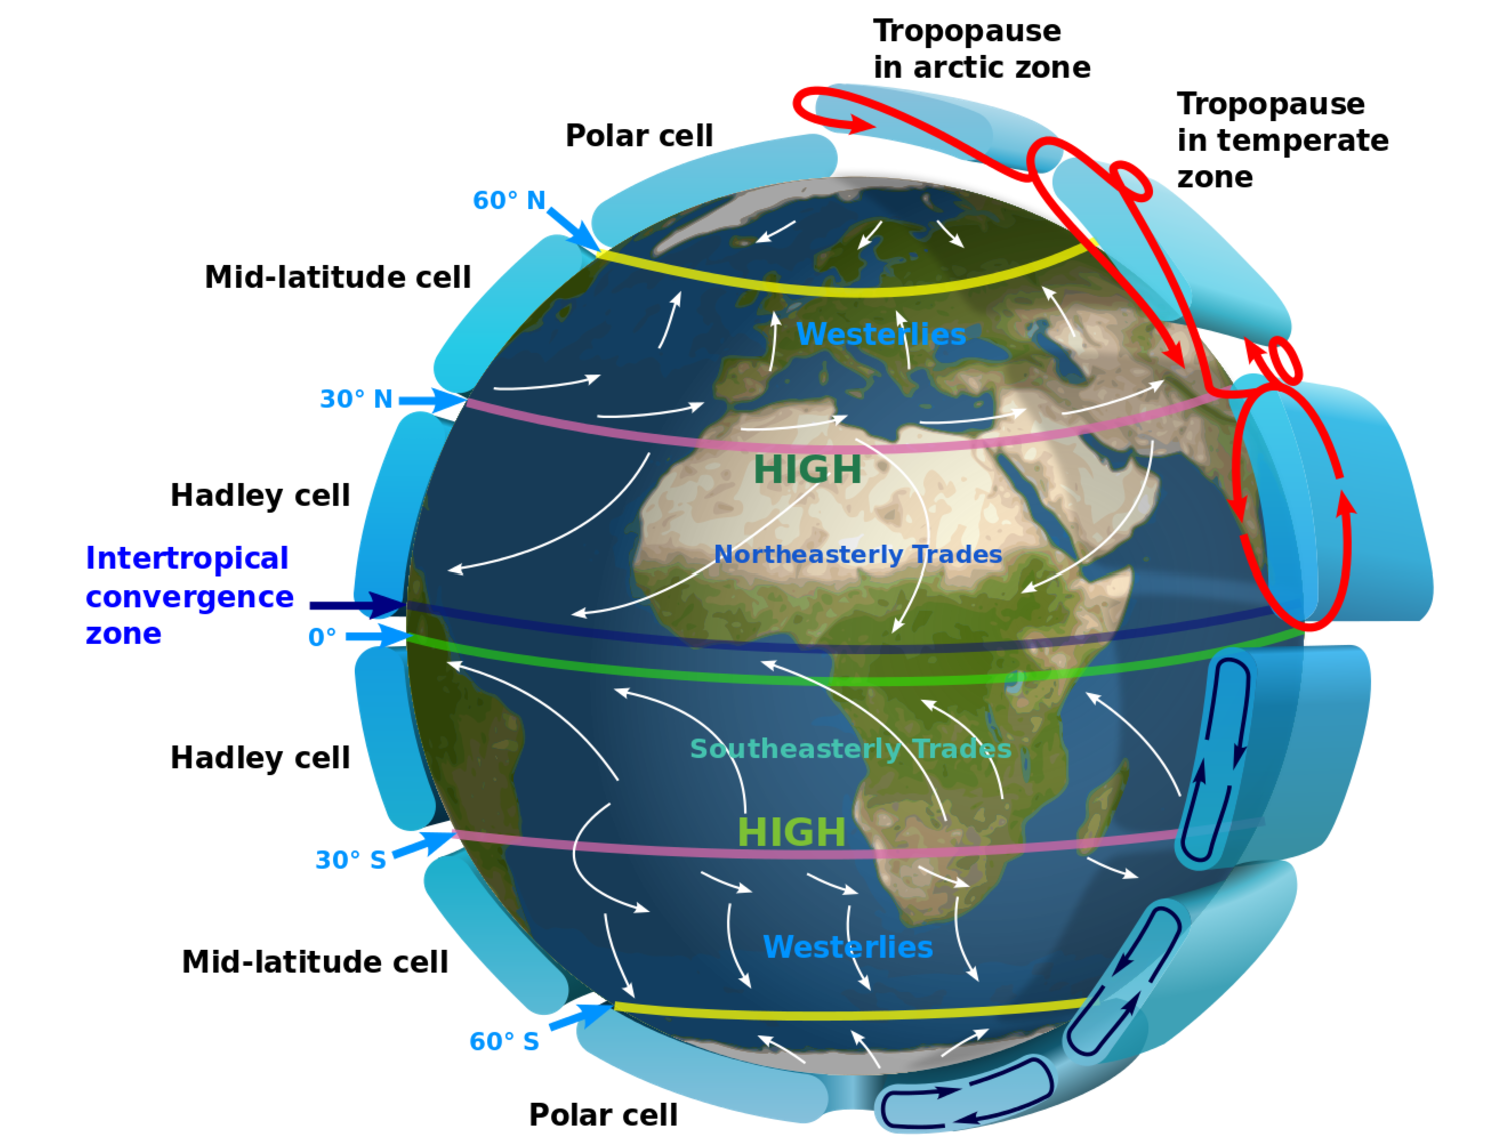
\includegraphics[width=0.5\linewidth]{upload/GAC.png}
	\caption{Global Atmospheric Circulation cells}
	\label{fig:GAC}
\end{figure}

In reality, the atmospheric circulation is more complex than the three-cell model suggests. It exhibits significant temporal and spatial variations due to factors like land/sea contrasts, topography, and changes in solar heating. While the model serves as a foundational framework, modern climate science relies on satellite data and simulations for a detailed understanding of global atmospheric dynamics.



\paragraph{Monsoons and Land Sea breezes:} they are wind patterns driven by differences in heating between land and water surfaces, but they operate on different scales.
\newline \textbf{Sea Breeze} (Daytime): During the day, land heats up faster than water, causing air over the land to rise and creating a low-pressure zone. Cooler, denser air from over the sea flows in to replace it, generating a breeze from sea to land.
\newline \textbf{Land Breeze}(Nighttime): At night, the land cools faster than water, creating a high-pressure zone over the land. Air flows from the land to the sea, forming a weaker land breeze.
\newline \textbf{Summer Monsoon}: Similar to a large-scale sea breeze, during summer, land masses (like South Asia) heat up more quickly than the surrounding oceans. This creates a low-pressure zone over land, drawing in moist air from the Indian or Pacific Oceans. The moisture-laden air rises and cools, resulting in heavy rainfall, particularly over mountain ranges like the Himalayas and Ghats.
\newline \textbf{Winter Monsoon}: In winter, the land cools faster than the ocean, forming a high-pressure zone. Cold, dry air flows outward from the land to the sea, leading to dry weather conditions over most of South Asia.
\newline Key Differences:while land/sea breezes are localized and operate on a daily cycle, monsoons occur over larger areas and are seasonal, driven by shifts in the Intertropical Convergence Zone (ITCZ).
Monsoons involve additional complexities, including the influence of upper atmospheric circulations, such as the jet stream.
The Asian monsoon, particularly over South Asia, is the most prominent example, crucial for regional agriculture and ecosystems. However, its dynamics are far more complex than those of simple land and sea breezes.

\subsection{The time averaged zonal general circulation}
The time-averaged circulation, computed from ERA5 Reanalysis data, shows westerly mid-atmosphere jets in the subtropical regions of both hemispheres. These jets reach a maximum around the 200mb level (\~12 km) and extend to the surface in the mid-latitudes, while easterly flows dominate the equatorial zone. The jets exhibit a strong seasonal cycle, with accelerated jets in winter and weaker jets in summer. There is a seasonal poleward migration of the jet cores, with the winter season showing more concentrated and intense maximums. The Southern Hemisphere's winter jet is broader than its Northern Hemisphere counterpart, both linked to the stratospheric flow above.

The stratosphere also exhibits strong jets with a stronger seasonal cycle, where easterlies replace westerlies as the seasons change. In the meridional circulation, low-level convergence occurs at the equator, with high-level divergence. The InterTropical Convergence Zone (ITCZ) oscillates between 15°N and 5°S, influenced by the seasonal cycle of the sun.

Temperature decreases with latitude due to radiation balance, with the equator receiving more solar radiation than the poles. The temperature decreases with height in the atmosphere, though the lapse rate is less than adiabatic, indicating a generally stable atmosphere. There is a strong latitudinal temperature gradient, which weakens with altitude and reverses in the upper atmosphere and stratosphere, due to radiation absorption by ozone and other components in the lower stratosphere.

The reversal of the meridional temperature gradient aligns with the zonal wind structure, showing positive shear in the troposphere and negative shear above, consistent with thermal wind balance. Water vapor, measured as specific humidity, is concentrated in the lower atmosphere and the equatorial region, with significant dryness at higher altitudes. The atmosphere's moisture content decreases with altitude due to the Clausius-Clapeyron relation, which links water vapor pressure to temperature. At the equator, moist air contains 12-15 grams of water per kilogram of air.

Specific humidity follows the seasonal cycle of the sun, shifting latitudinally. The maximum is located around 5°S in December-February (DJF) and around 10°N in June-July-August (JJA). The winter hemisphere is more moist at the surface than the summer, though values in the winter are smaller than in the equatorial zone, reaching up to 8 g/kg.

\subsection{The horizontal general circulation and wind }

The climatological geopotential height at 200mb shows deviations from a zonally symmetric circulation, particularly over the east coasts of continents, downstream from major mountain ranges like the Rockies and Himalayas. These features are clearer with specialized projections, highlighting the winter atmospheric pattern. While geopotential height can approximate wind flow in mid-latitudes, wind analysis is more useful in low latitudes.

At 200mb, winter jet streams are strong in both hemispheres, especially over Asia, with the Asian jet reaching velocities over 70 m/s. The Southern Hemisphere jet is weaker. In summer, westerly jets are weaker, and easterly jets dominate the tropics. The Indian Ocean sees a strong easterly flow in summer, leading to divergence over South America and Indonesia.

The meridional wind shows alternating poleward and equatorward patterns in winter, with large deviations in the Pacific-North American sector and East Asia. In summer, winds weaken but remain stronger in the Southern Hemisphere. Near the surface, the zonal wind is stronger over oceans and weaker over land, with easterlies in the subtropics, except in the Indonesian region, where westerlies prevail. The equatorial Pacific shows a convergence zone.

During JJA, the seasonal cycle strengthens winter wind features, with strong westerlies in the Indian Ocean signaling the start of the South Asian Monsoon. The meridional wind shows an equatorward flow along continent coasts, intensifying in summer, and reversing along the Somali coast.

At the 850mb level, trade winds dominate the equatorial Pacific, shifting with the ITCZ’s seasonal cycle. The Asian Summer Monsoon is visible in the Indian Ocean, forming a large gyre from East Africa to the Indian subcontinent, crucial for understanding low-level atmospheric and oceanic interactions.

\subsection{Mean Sea Level Pressure and The Sea Surface Temperature}
(MSLP) is a key parameter in describing atmospheric circulation. It represents the atmospheric pressure adjusted to mean sea level, though its usefulness is limited in areas with significant mountains, like the Rockies, Himalayas, and Antarctica, where the concept of "sea level" is effectively underground. Outside these areas, MSLP provides a good representation of atmospheric mass distribution. High MSLP areas correspond to mass accumulation, particularly in the subtropics, where high-pressure systems are common in both summer and winter.

Near-surface temperatures, typically measured 2 meters above the ground, reflect the seasonal and geographical variation in temperature. Over oceans, they follow sea surface temperature (SST), but land areas show significant seasonal changes. Northern continents are colder than the oceans at the same latitude, and coastal regions also experience temperature differences, with west coasts being milder than east coasts. In winter, high pressure tends to remain over land while low pressure develops over the oceans, reversing in summer. The intertropical zone sees high-pressure centers shifting with the seasons, while the Southern Hemisphere features a more symmetric pattern, with a ring of low pressure around Antarctica.

The seasonal cycle is evident in the shift of high-pressure areas in the tropics, moving latitudinally with the changing seasons. The meridional distribution of sea level pressure shows high pressure in the tropics, with low pressure areas near the equator and in the mid-latitudes. In the Southern Hemisphere, the pressure gradients are stronger and more pronounced, with tropical pressure maxima shifting seasonally.

Sea Surface Temperature (SST) shows strong north-south gradients, with polar regions being cold and the equator generally warm. However, notable deviations from zonal symmetry occur near continental east coasts, particularly in the equatorial Pacific, where cold water intrudes at the equator in the East Pacific, contrasting with the warm waters of the West Pacific. These temperature differences highlight significant gradients in SST along the equator



\subsection*{The Role of Energy Processes}

The vertical temperature gradient in the atmosphere is maintained by complex energy processes, including the absorption and radiation of heat, convection, and interactions with the Earth's surface. These processes vary with latitude and season, creating the dynamic and layered structure of the atmosphere.

Inversions, which occur when surface air cools significantly, disrupt the usual temperature gradient, particularly in the troposphere. These events highlight the intricate balance of energy transfer within the atmosphere and its impact on weather and climate.

\subsubsection{Energy balances }
To understand how the atmosphere maintains the various temperature structures, it is necessary to consider the processes by which the atmosphere gains and loses energy and how these processes vary with latitude and season. Essentially all the energy that enters in the climate system comes from the sun, part of it is absorbed in the system and must be balanced with outgoing energy leaving the system, to maintain the overall climate system in its observed equilibrium state.

Because of the different temperatures between the sun and the Earth, the energy emitted by the two bodies is sharply different. The spatial and temporal distribution of the receipt of solar energy at the Earth’s surface is highly dependent upon the Earth's annual revolution around the sun, its daily rotation about its axis, and the tilt of its axis concerning the plane of its orbit.

When the Earth is in the portion of its orbit where the Northern Hemisphere is tilted toward the sun, the Northern Hemisphere receives the majority of the direct sunlight and experiences summer, while the Southern Hemisphere experiences winter. Naturally, the reverse occurs when the Earth is in the opposite portion of its orbit, with the Southern Hemisphere tilted toward the sun.

About half of the incoming solar radiation is absorbed by the Earth's surface. This energy is transferred to the atmosphere by warming the air in contact with the surface (sensible heat), by evaporation and by thermal radiation that is absorbed by clouds and by greenhouse gases. The atmosphere in turn radiates thermal radiation back to Earth as well as out to space. Since all the
incoming radiation equals to $342 \,\, \text{Wm}^{-2}$ and $107 \,\, \text{Wm}^{-2}$ of it is reflected back to space, there must be
$235\,\, \text{Wm}^{-2}$ of terrestrial radiation emitted to space for an equilibrium situation from three main sources: water vapor, $CO_2$, clouds and Earth’s surface.

At the top of the atmosphere, the energy balance is composed of the compensating fluxes between the incoming solar radiation and the outgoing thermal radiation from the Earth. The solar radiation will be modulated by the reflectivity caused by the atmospheric cloud and in smaller part by the molecular components of the atmosphere itself. The thermal radiation will be modulated by the absorption properties of the atmosphere and its constituents. Both will be affected by the circulation and ultimately by the atmospheric flows.

The net balance shows a surplus of radiative flux in the subtropical region and a deficit in the polar regions. The global radiation budget can be obtained by integrating over the surface of the Earth the radiative fluxes.

At the surface, the energy balance involves more processes. There is also here a net solar radiation flux, modulated by the albedo of the surface and of the atmosphere, and a net thermal flux, obtained as the balance between the radiation emitted by the surface and the downward flux coming from the bulk of the atmosphere. Then there is a sensible heat flux caused by the turbulent vertical motion that carries away heat through mechanical agitation and the latent heat flux that represents the heat necessary for the evaporation of water from the surface. Because of the extent of the ocean, the latent heat flux is an important element of the budget.

In addition, we can look at the total cloud cover which is essentially the aggregated quantity of clouds at various levels. This is the quantity that is intuitively linked to the observation of a “cloudy sky”. In general, clouds are present over a vast surface of the globe. Some areas show a persistent absence of cloudiness over the entire year, such as the Sahara desert, part of the Arabian peninsula, Australia, and South Africa. Other areas instead show a strong seasonal cycle, with different could cover in different seasons. It is interesting to note that the seasonal cycle takes different characteristics in different areas. In the mid-latitudes cloud cover is larger in the local hemispheric winter than in the summer.

Looking at the zonal profile of the clouds, it is evident that major concentrations are related to the equator and middle/high latitudes.



\section{Oceans}
Oceans, covering approximately 71\% of Earth's surface, play a crucial role in global climate systems by storing and transferring heat, nutrients, and momentum. The interaction between the atmosphere and oceans significantly impacts weather and climate patterns. These bodies of water contain an estimated 1,350 million cubic kilometers of water, predominantly found in the Pacific, Atlantic, Arctic, and Southern Oceans, with an average depth of about 4,000 meters.
\newline Surrounding continents are continental shelves, shallow areas that extend outward for several kilometers before dropping sharply at the continental slope into the deep ocean floor. The ocean floor itself is varied, featuring features like underwater mountains, ridges, trenches, and smooth sedimentary basins.
\newline The oceans redistribute solar energy from equatorial to higher latitudes. As water warms at low latitudes, it absorbs significant amounts of solar heat. This heat is released into the atmosphere in the form of latent heat and longwave radiation as water cools or condenses, influencing global atmospheric circulation. Ocean currents further distribute this heat, balancing regional temperatures and aiding in climate regulation.(*)
\paragraph{Composition.} Seawater is not just water but a mixture containing various dissolved salts, with an average salinity of 35 grams per kilogram of water. This salinity largely comes from chloride, sodium, and sulfate, accounting for the majority of dissolved material. Salinity levels, however, vary globally. The Arctic Ocean shows lower salinity (~29\%), influenced by melting ice and freshwater inflows, while the subtropical Atlantic has some of the highest salinities (~37.5\%), due to high evaporation and low precipitation. These variations affect density, which in turn drives ocean circulation and temperature dynamics.
Overall, oceans are not only a storage medium for heat and nutrients but also critical in redistributing energy across the planet, moderating climate, and supporting ecosystems. Their interaction with atmospheric processes underscores their integral role in Earth's environmental systems.
\paragraph{Temperatures profiles.}
\subparagraph{Surface Temperatures:}
Range: -1°C (polar regions) to 20–30°C (tropics).
Seasonality: temperatures align in east-west zonal patterns, with exceptions like:
\begin{itemize}
	\item Tropical Pacific: western regions warmer than eastern regions due to currents.
	\item Gulf Stream: transports warm water northeast, moderating European climates.
\end{itemize}

\subparagraph{Temperature with Depth:}
\begin{itemize}
	\item Mixed Layer ($0–30$ m in summer):
	      warmed by sunlight and mixed by winds.
	\item Thermocline ($200–1000$ m):
	      sharp temperature gradient separating surface water from deeper layers.
	\item Deep Ocean ($>1000$ m):
	      uniform cold temperatures ($0.5–1.25°$C).
	\item Coldest water ($-0.25°$C) near Antarctica due to sinking dense, salty water from surface cooling and sea ice formation.
\end{itemize}

\begin{wrapfigure}{R}{0.5\textwidth}
	\begin{center}
		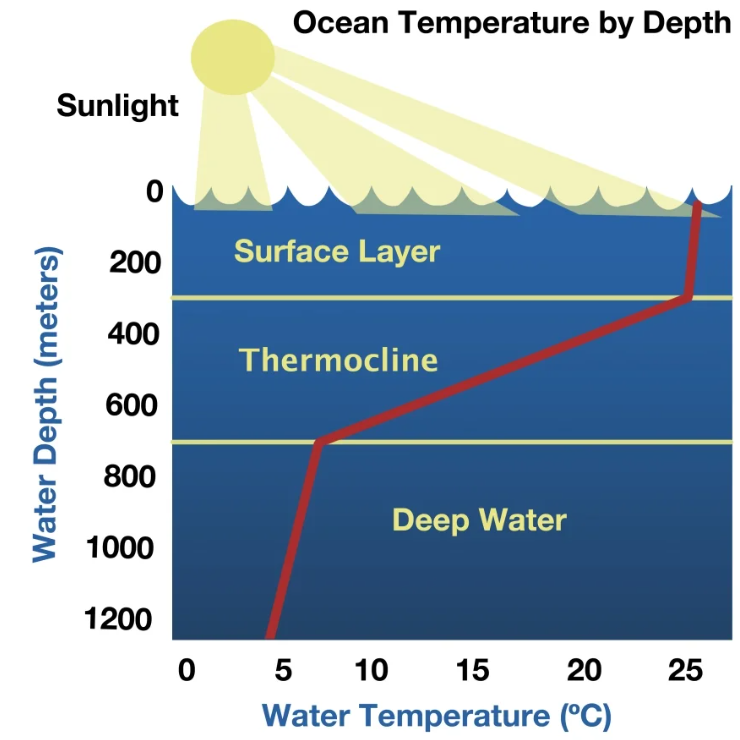
\includegraphics[width=0.3\textwidth]{upload/Ocean T.png}
	\end{center}
	\caption{Ocean temperature diagram (unprecised values on the $y$-axis)}
	\label{}
\end{wrapfigure}



Ocean circulation is driven by temperature and salinity differences, influencing density and pressure. Surface currents are wind-driven, forming large gyres such as those in the Pacific and Atlantic Oceans. These gyres redistribute heat and nutrients, shaping regional climates and ecosystems. Deep ocean currents, part of the thermohaline circulation\footnote{\url{https://rwu.pressbooks.pub/webboceanography/chapter/9-8-thermohaline-circulation/}}, involve the sinking of dense, cold water and the upwelling of warmer, nutrient-rich water, critical for sustaining marine life.
Additionally, mesoscale eddies, swirling water masses, play a significant role in transporting momentum, heat, and nutrients horizontally and vertically, although their dynamics are not fully understood. These processes together illustrate the complex and vital role oceans play in regulating Earth's climate and supporting life.
\begin{figure}[htbp]
	\centering
	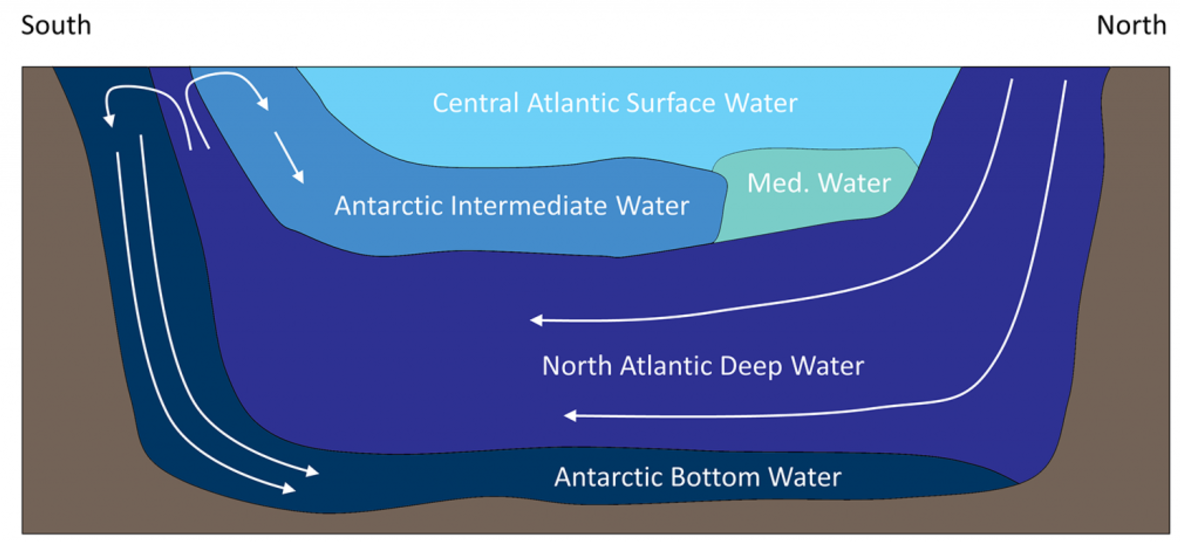
\includegraphics[width=0.5\linewidth]{upload/atlocean.png}
	\caption{The major water masses of the Atlantic Ocean}
	\label{fig:enter-label}
\end{figure}
\\
[0.1cm]

\subsection{The salinity structure of the ocean }
The salinity structure of the oceans is shown in Figure \ref{fig:fig1}.  The top panel shows the salinity near the surface at a nominal depth of
5m. We notice that there is a complex structure with low salinity
(fresher) waters at the poles and progressively more saline water moving towards the Equator, but then salinity decreases again at the equator. It is probably instructive to look at the latitudinal distribution of the precipitation. We can notice that the peaks of precipitation in the midlatitude and at the Equator are correlated with the low-salinity areas, whereas the subtropical regions are regions of strong evaporation, whose signature is the high salinity of the surface waters.

The Pacific Ocean is fresher than the Atlantic or even the Indian Ocean.
We can see from the map at 1000m that sources of saline waters are
marginal seas like the Mediterranean and the Persian Gulf. These areas
are evaporative basins that produce water so saline that it dominates
over the temperature effect and becomes denser so that we can find
Mediterranean water below the surface.
\begin{wrapfigure}{R}{0.5\textwidth}
	\begin{center}
		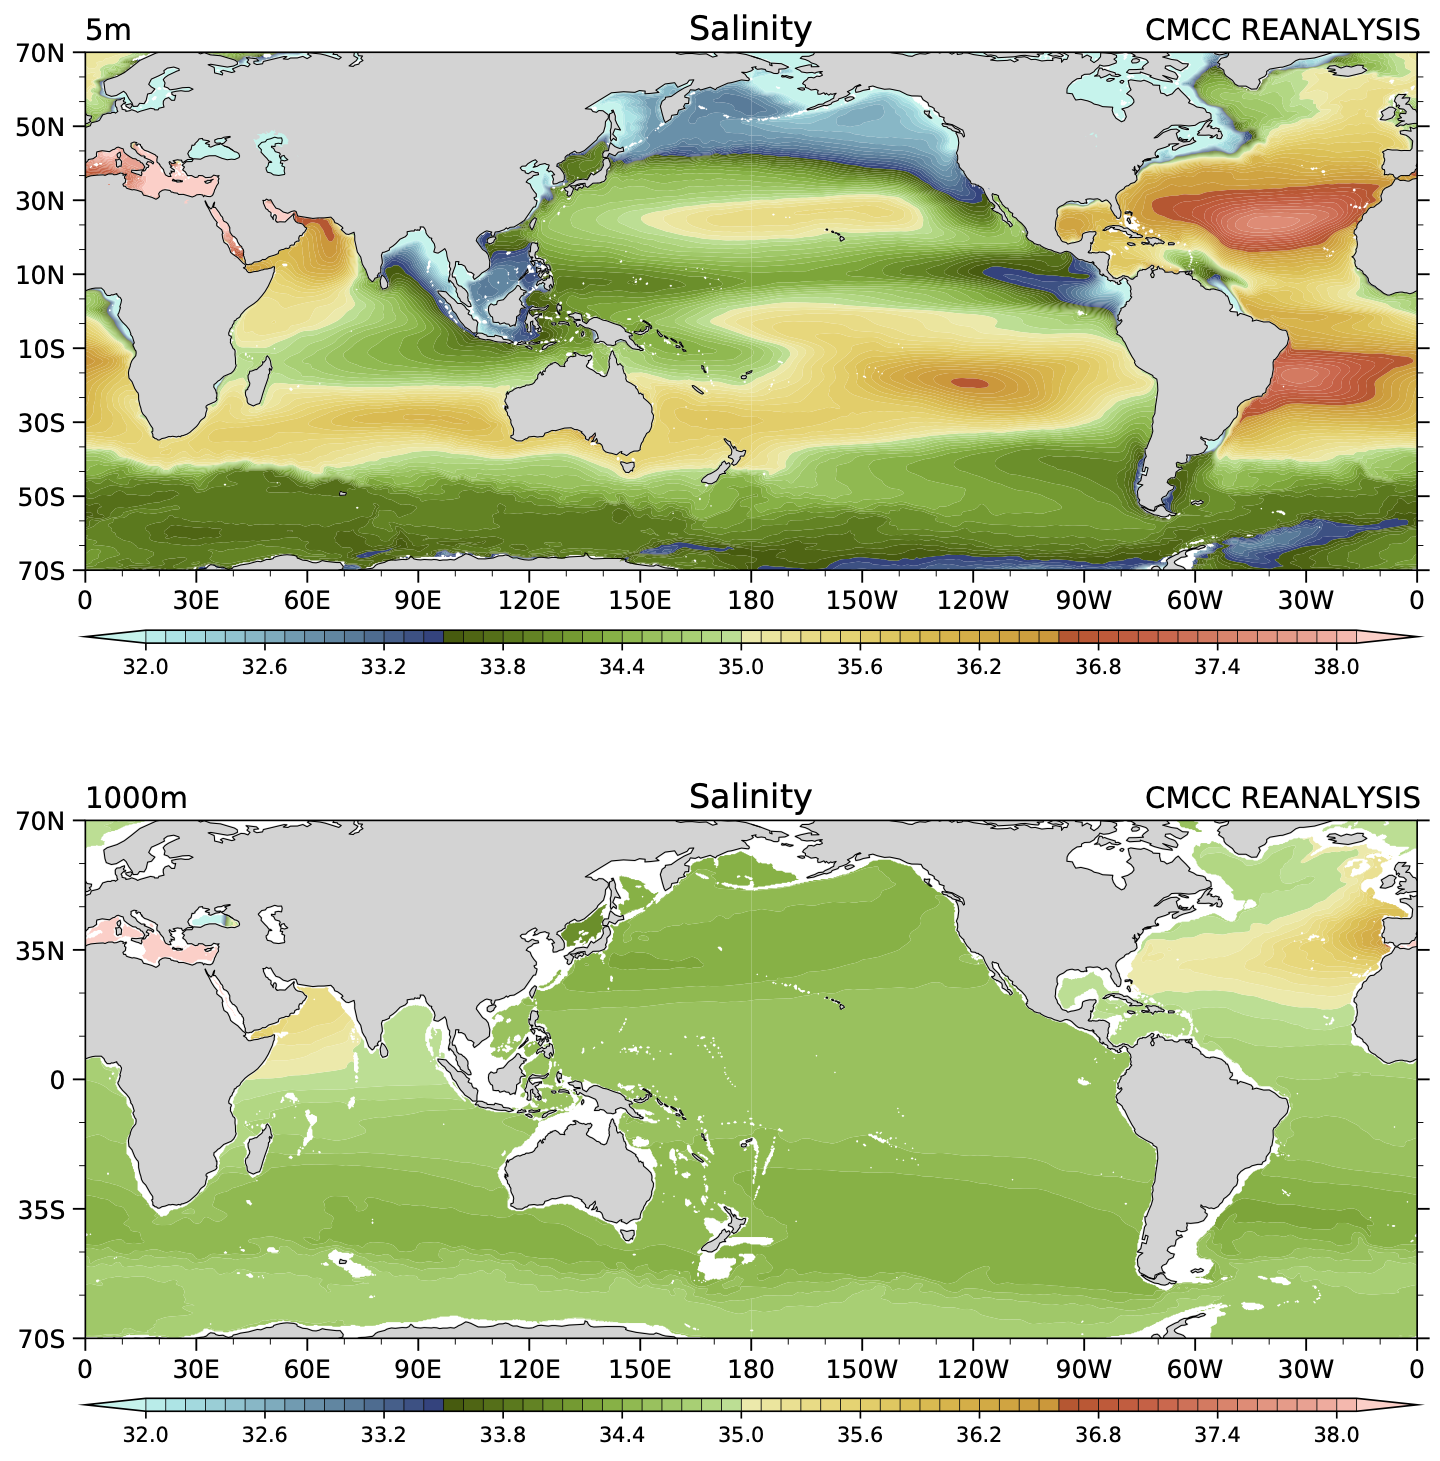
\includegraphics[width=0.48\textwidth]{upload/26image.png}
	\end{center}
	\caption{Salinity structure}
	\label{fig:fig1}
\end{wrapfigure}


The effect of the precipitation is less visible at the deeper depth pf
1000m (bottom panel), where the ocean tends to be fresher and more
uniform. We are using here the same scale to give a feeling of the
changes in salinity, except for the Atlantic and the east Indian Ocean,
the salinity is around 34 psu.
The effect of the runoff from major river systems is visible along the
Atlantic coast of South America where the Amazon river discharges and in the Bay of Bengal and around Indochina from the run-off the major rivers there, the Ganges and the Mekong.


In the pictures below: on the left salinity deviations with depth, going even deeper we have to change drastically
the scale. The oceans are remarkably uniform and the salinity deviations are really small. On the right, Pacific and Atlantic ocean salinity.



Looking at the North Atlantic (figures below) we notice that
there is a strong salinity gradient along the North American Coast that
follows roughly the pattern of the temperature gradient shown below. Strong temperature gradients are presumably to be
connected to the existence of currents, but we will need to check the
density, depending on the salinity later, to be sure.

\begin{minipage}{0.45\textwidth}\label{fig:fig4}
	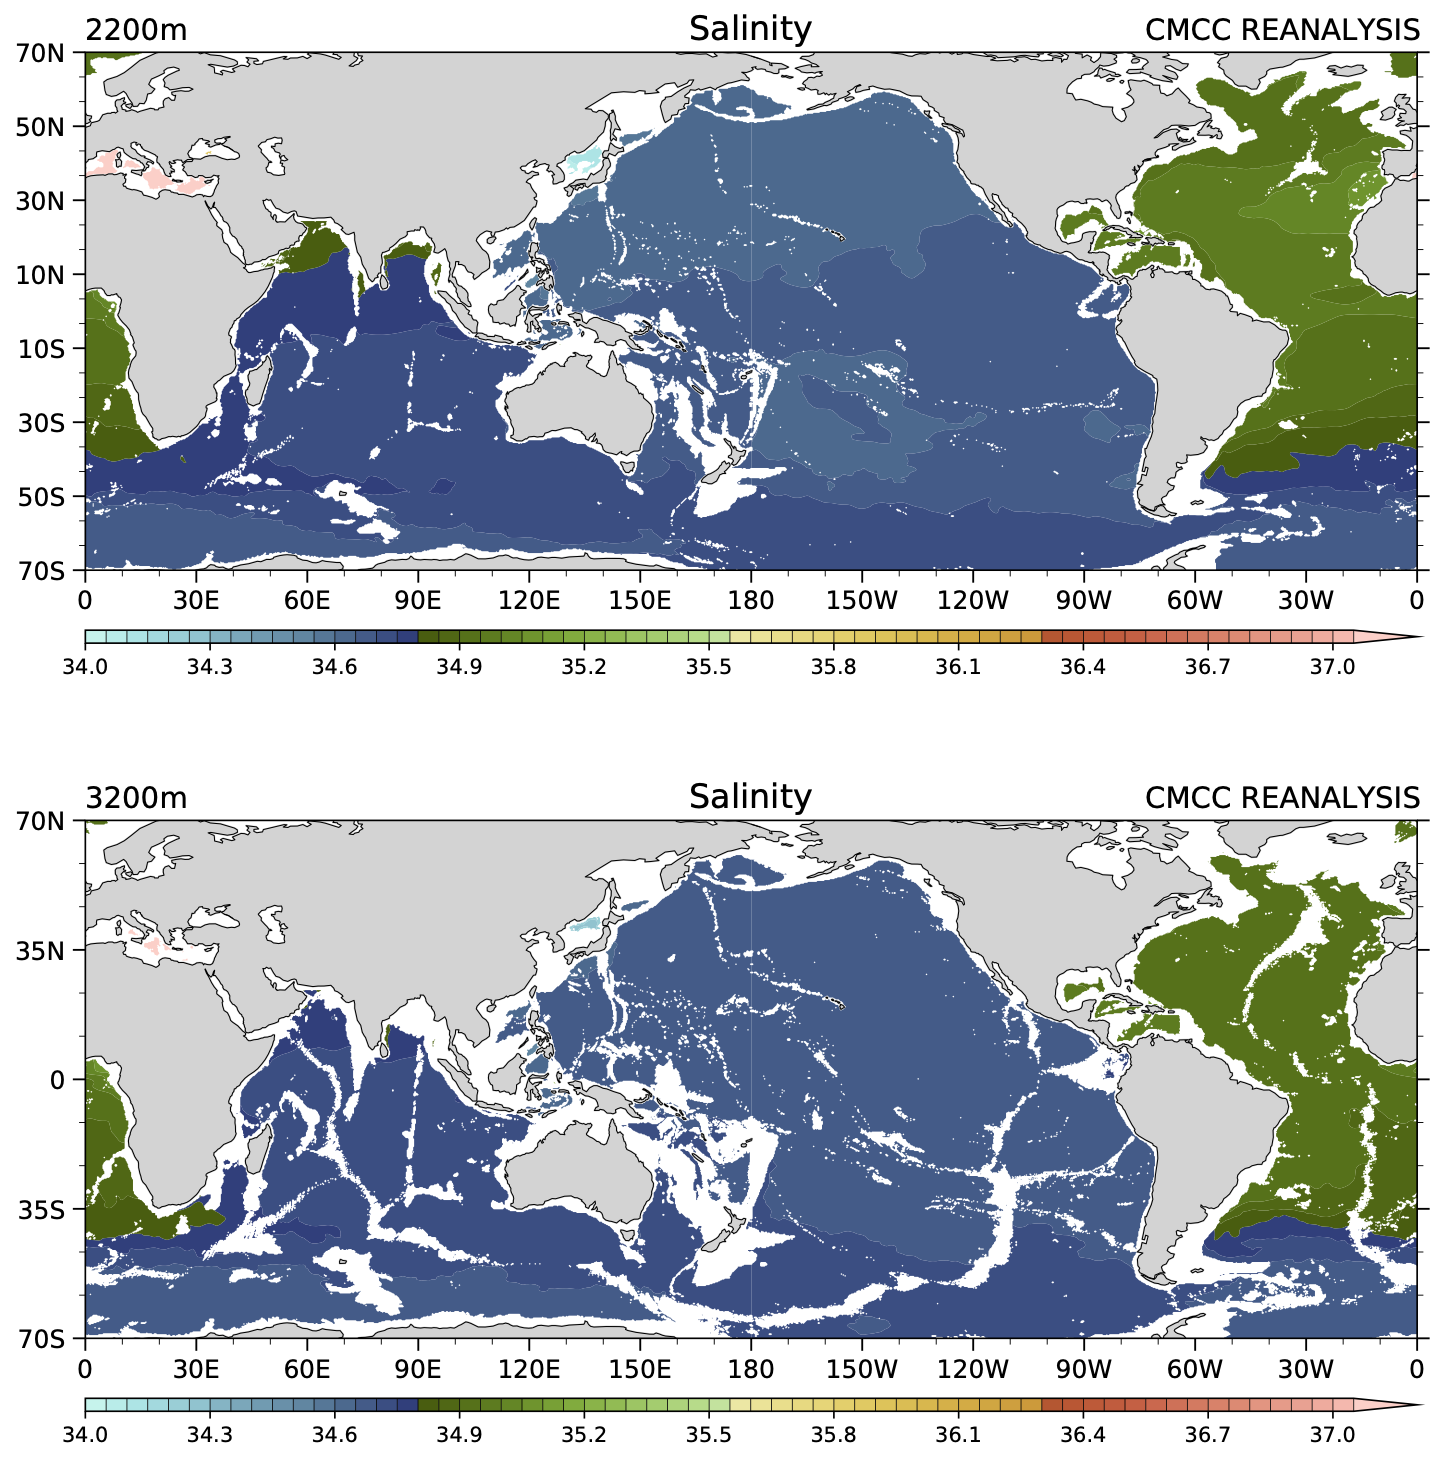
\includegraphics[width=0.9\textwidth]{upload/27image.png}
\end{minipage}
\begin{minipage}{0.45\textwidth}
	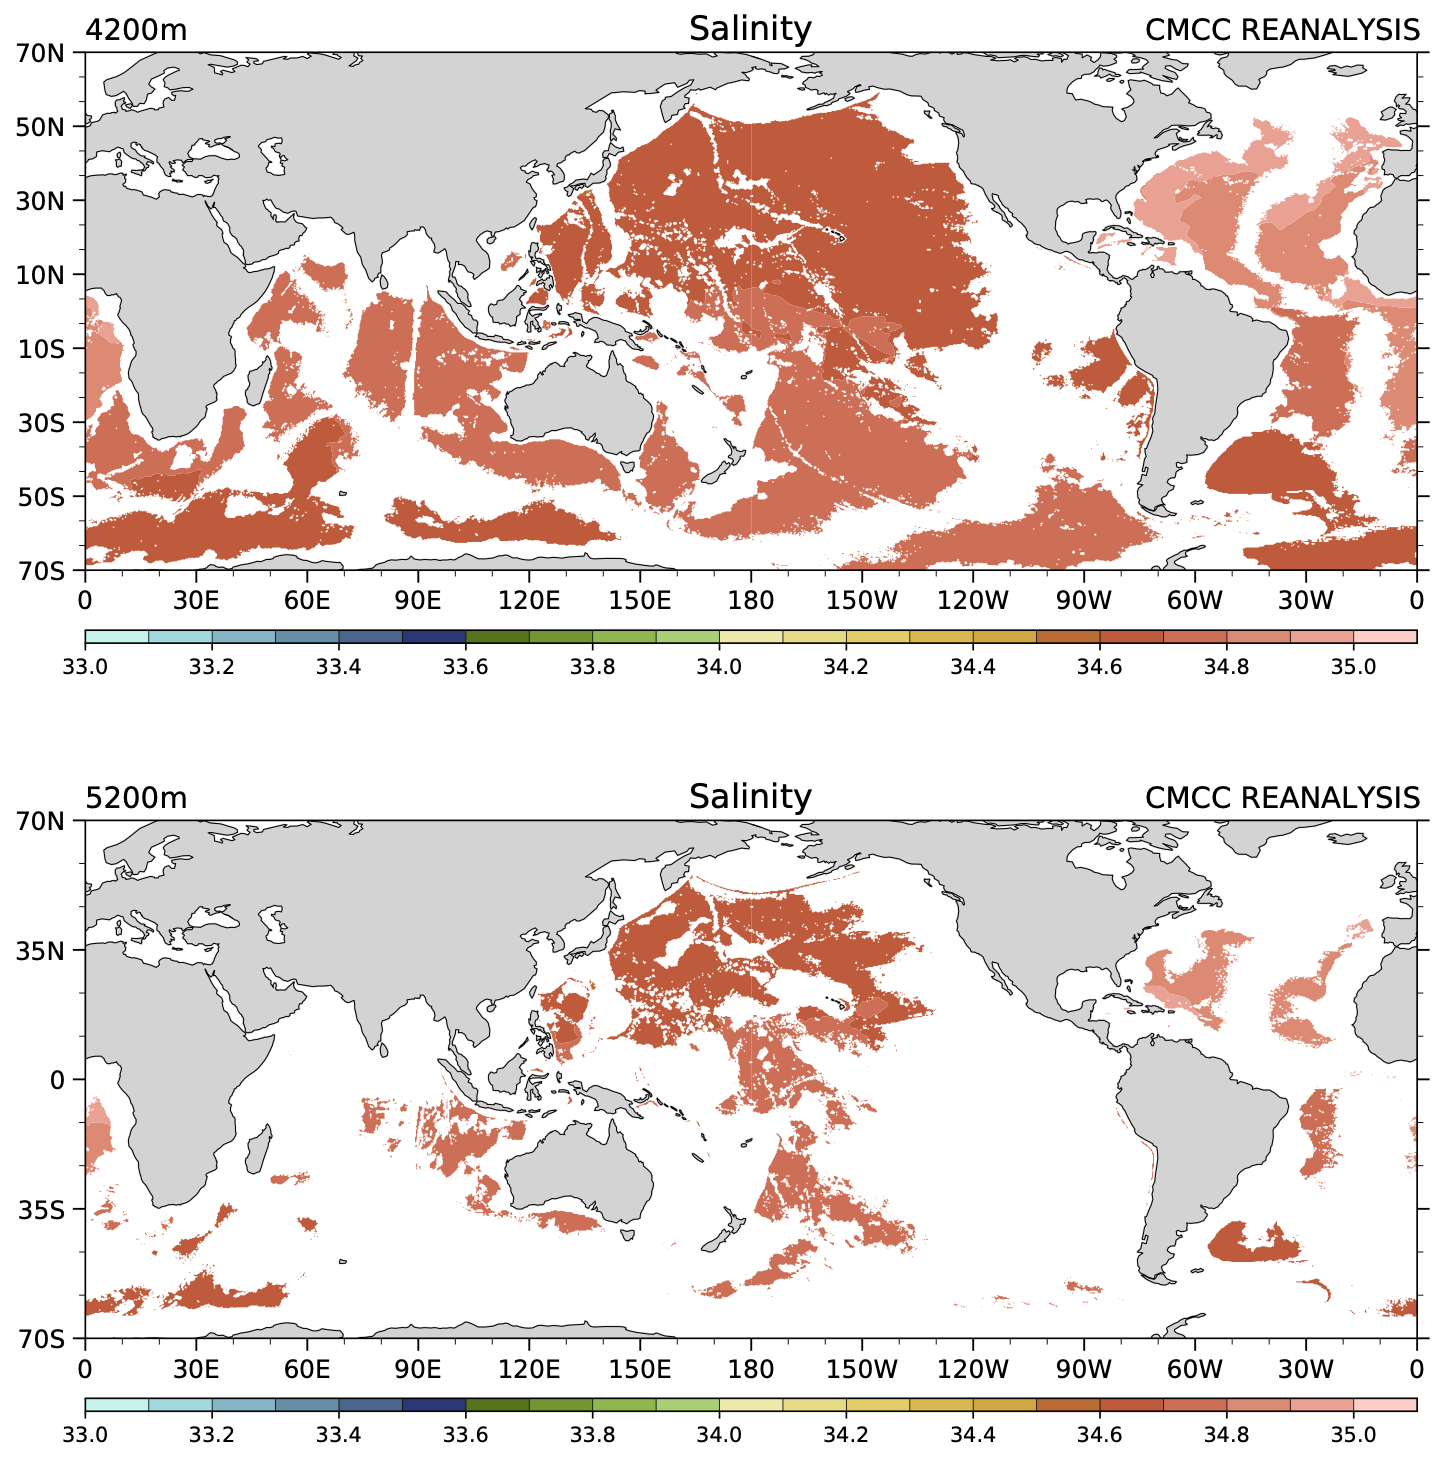
\includegraphics[width=0.9\textwidth]{upload/28image.png}
\end{minipage}\\
[0.1 cm]
Anyway,
this picture is giving a strong indication of the existence of something
remarkable and intense along the western boundary of the Atlantic ocean.


\begin{minipage}{0.45\textwidth}\label{fig:fig4}
	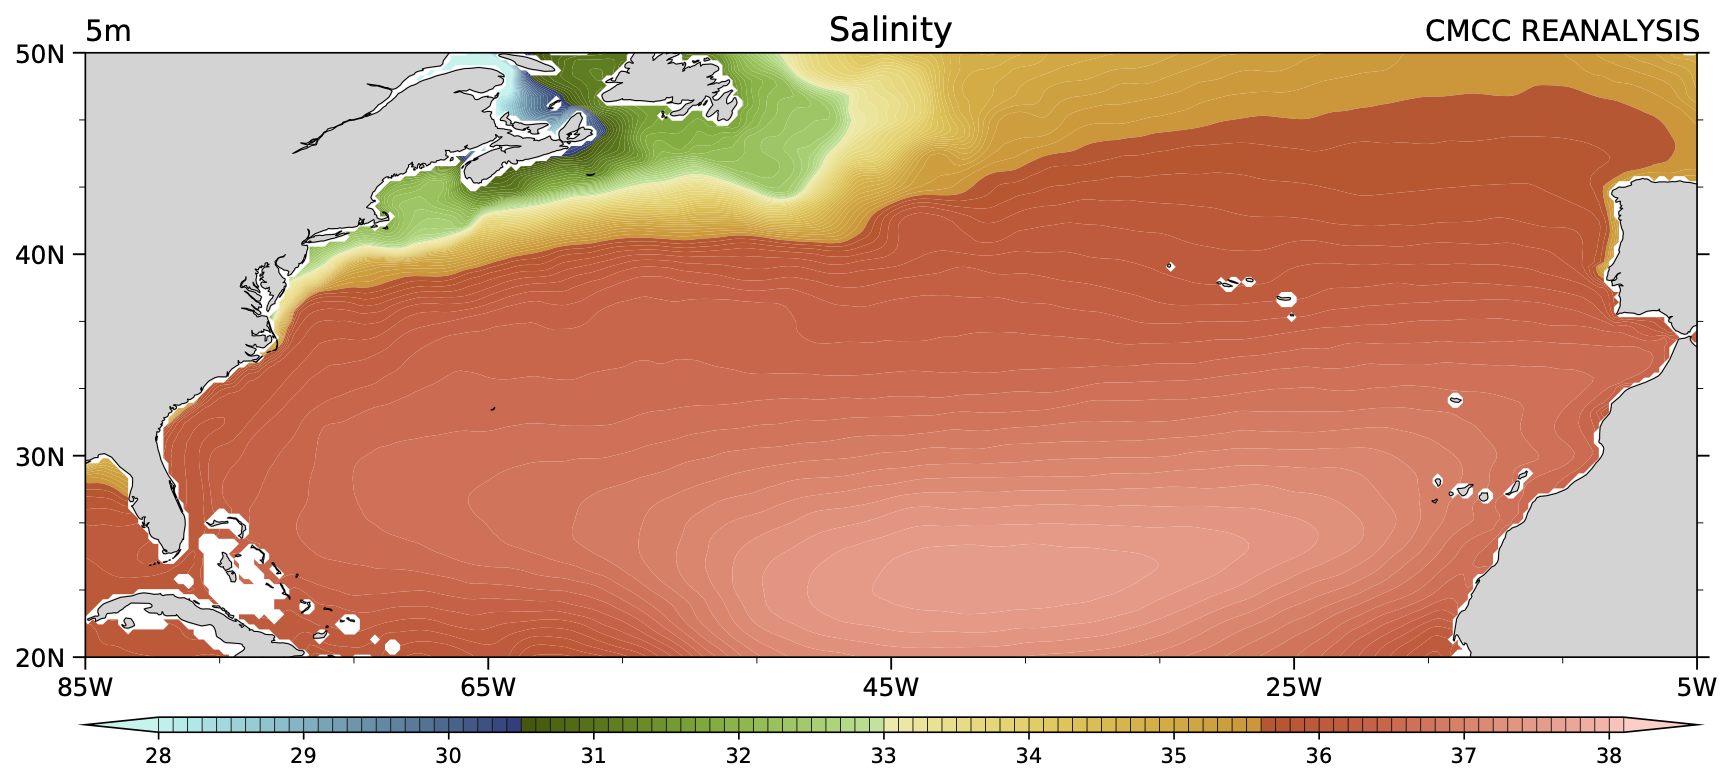
\includegraphics[width=0.9\textwidth]{upload/29image.png}
\end{minipage}
\begin{minipage}{0.4\textwidth}
	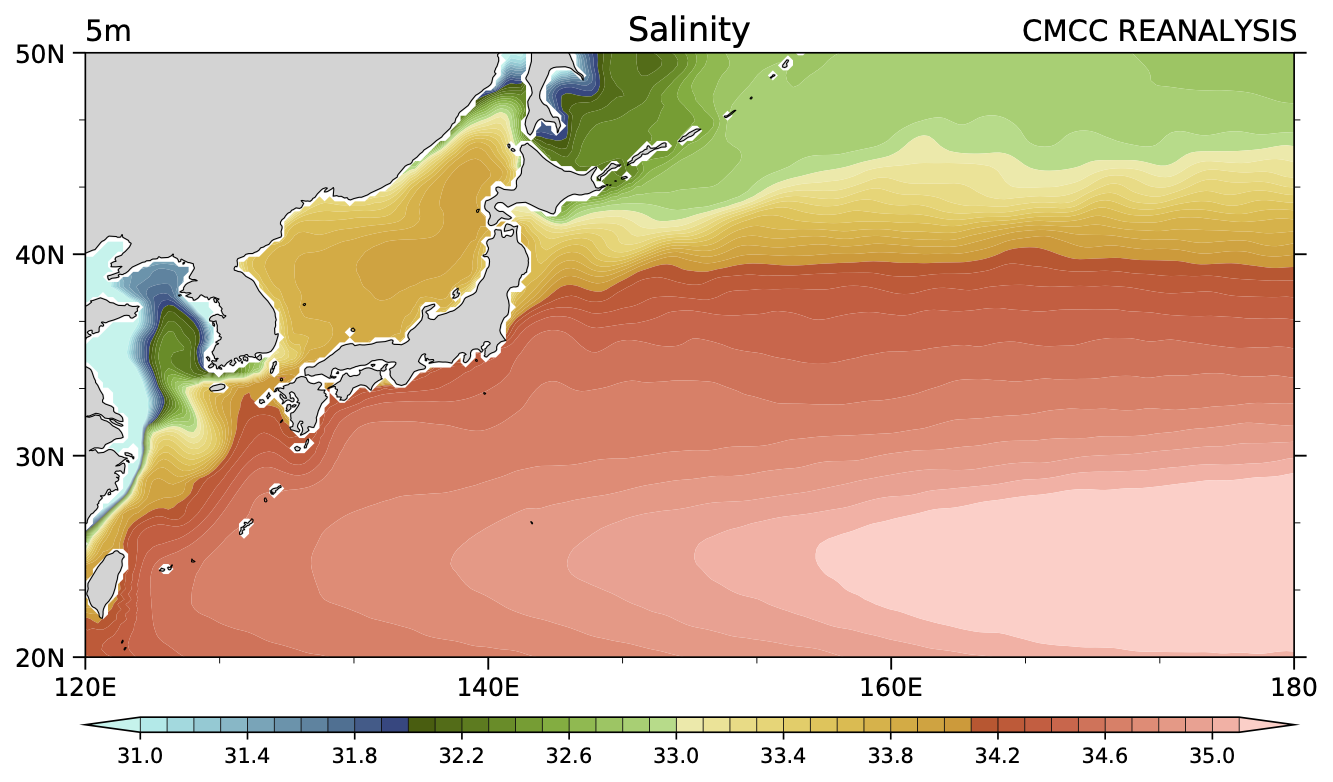
\includegraphics[width=0.9\textwidth]{upload/30image.png}
\end{minipage}\\


A similar situation exist in the North Pacific along the Japan coast and
therefore we can start to suspect that this has to do with the presence
of the continental boundary.

The previous analysis of the temperature is giving us hints of a strong
vertical structure of the oceans, so it may be useful to look at the
vertical distribution somewhat more in detail. The figures above show the same section North-South section of along the longitude of 25W, roughly in the middle of the Atlantic Ocean.
The salinity follows a similar pattern as the temperature with a
strong gradient approximately at the thermocline, the high salinity is
confined in thin; layers at the surface, but some interesting behaviour
is visible below. In the Northern Hemisphere we can see the
Mediterranean water penetrates at depth and actually protruding under the fresher water of Antarctic origin that is colder, but because is
fresher floats over the Mediterranean water. Really cold Antarctic water reaches the bottom, filling the abyssal plains of the basin.

\begin{figure}[htpb!]
	\centering
	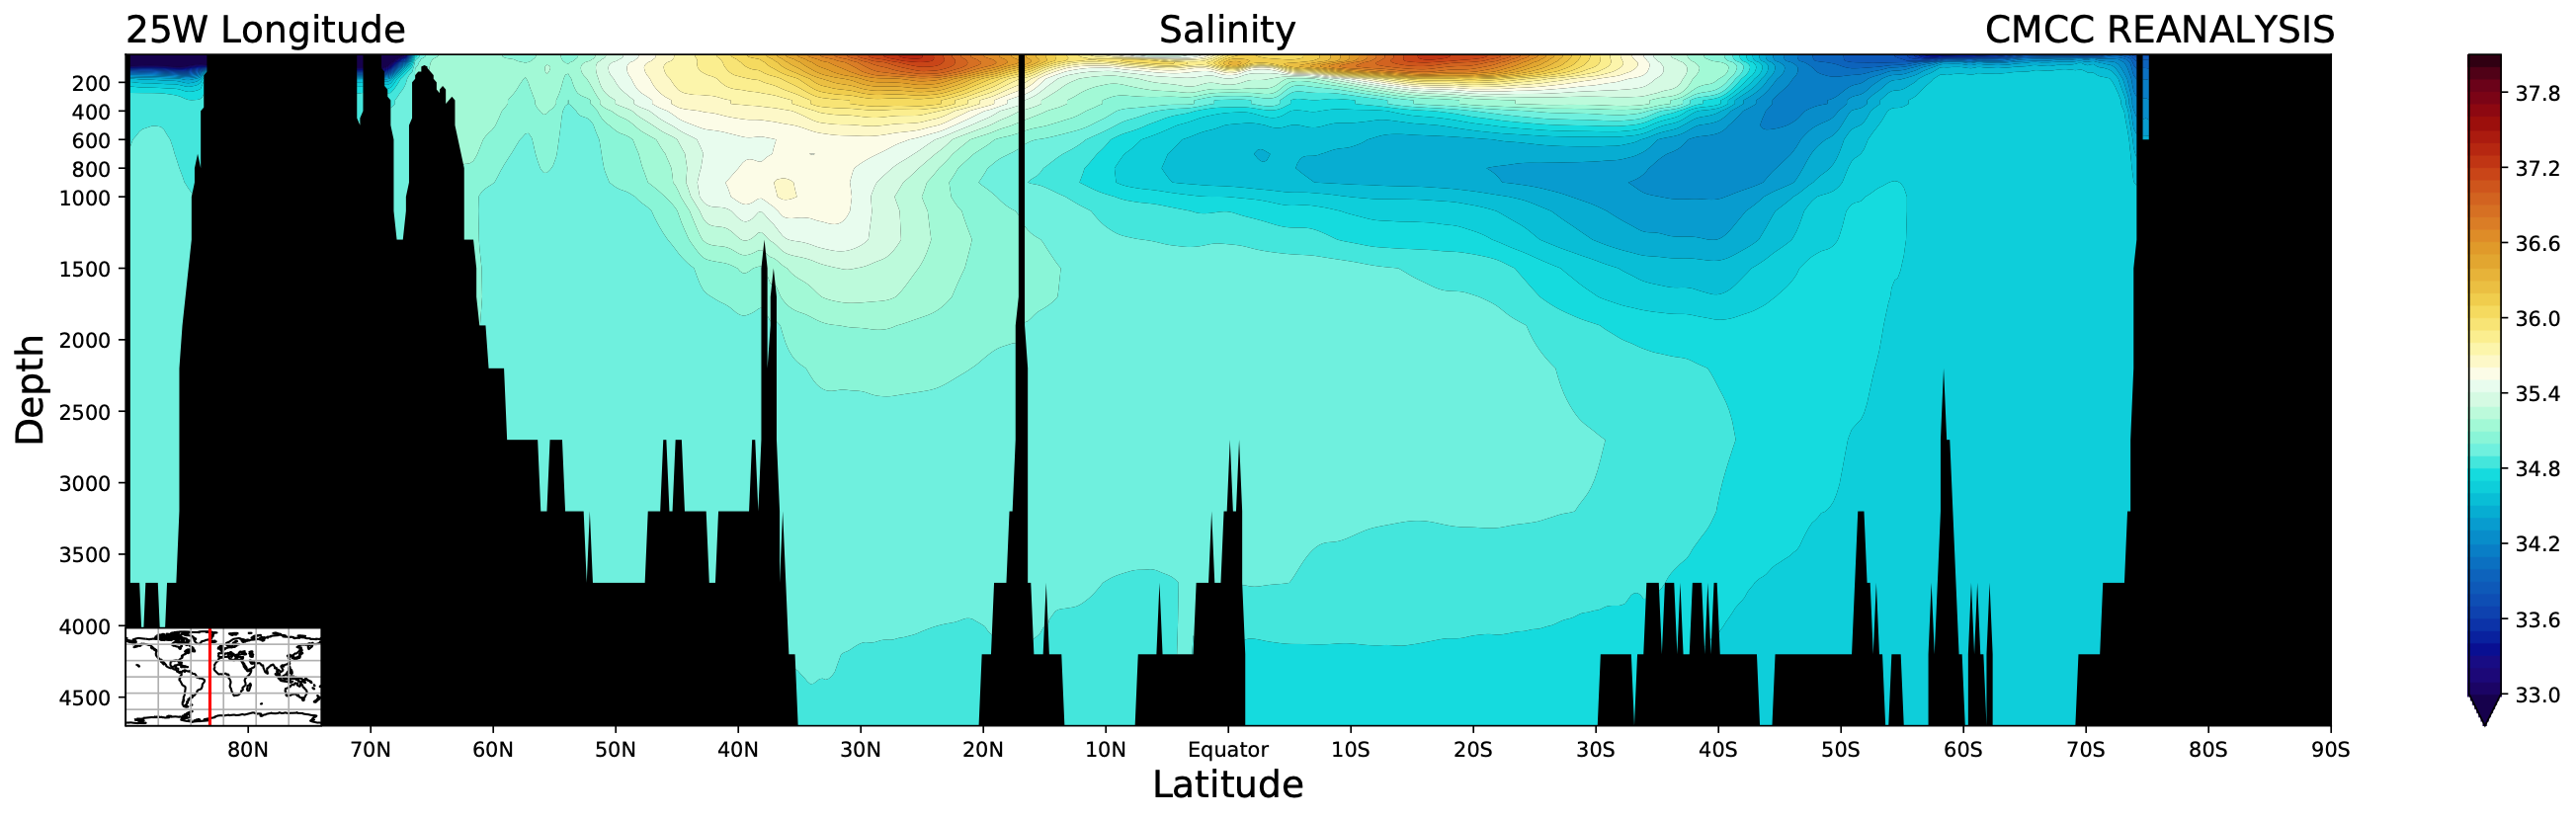
\includegraphics[width = 0.5 \textwidth]{upload/31image.png}
	\caption{North-South Salinity section at 25W longitude.}
	\label{fig:fig6}
\end{figure}

The Mediterranean waters are clearly visible in a longitude-depth
section (Figure \ref{fig:fig6}). The saline mediterranean water sinks
to about 1000m because it is warmer than the Atlantic but much more
saline so it is denser and it reaches an equilibrium depth at about
1000m.

\begin{figure}[htpb!]
	\centering
	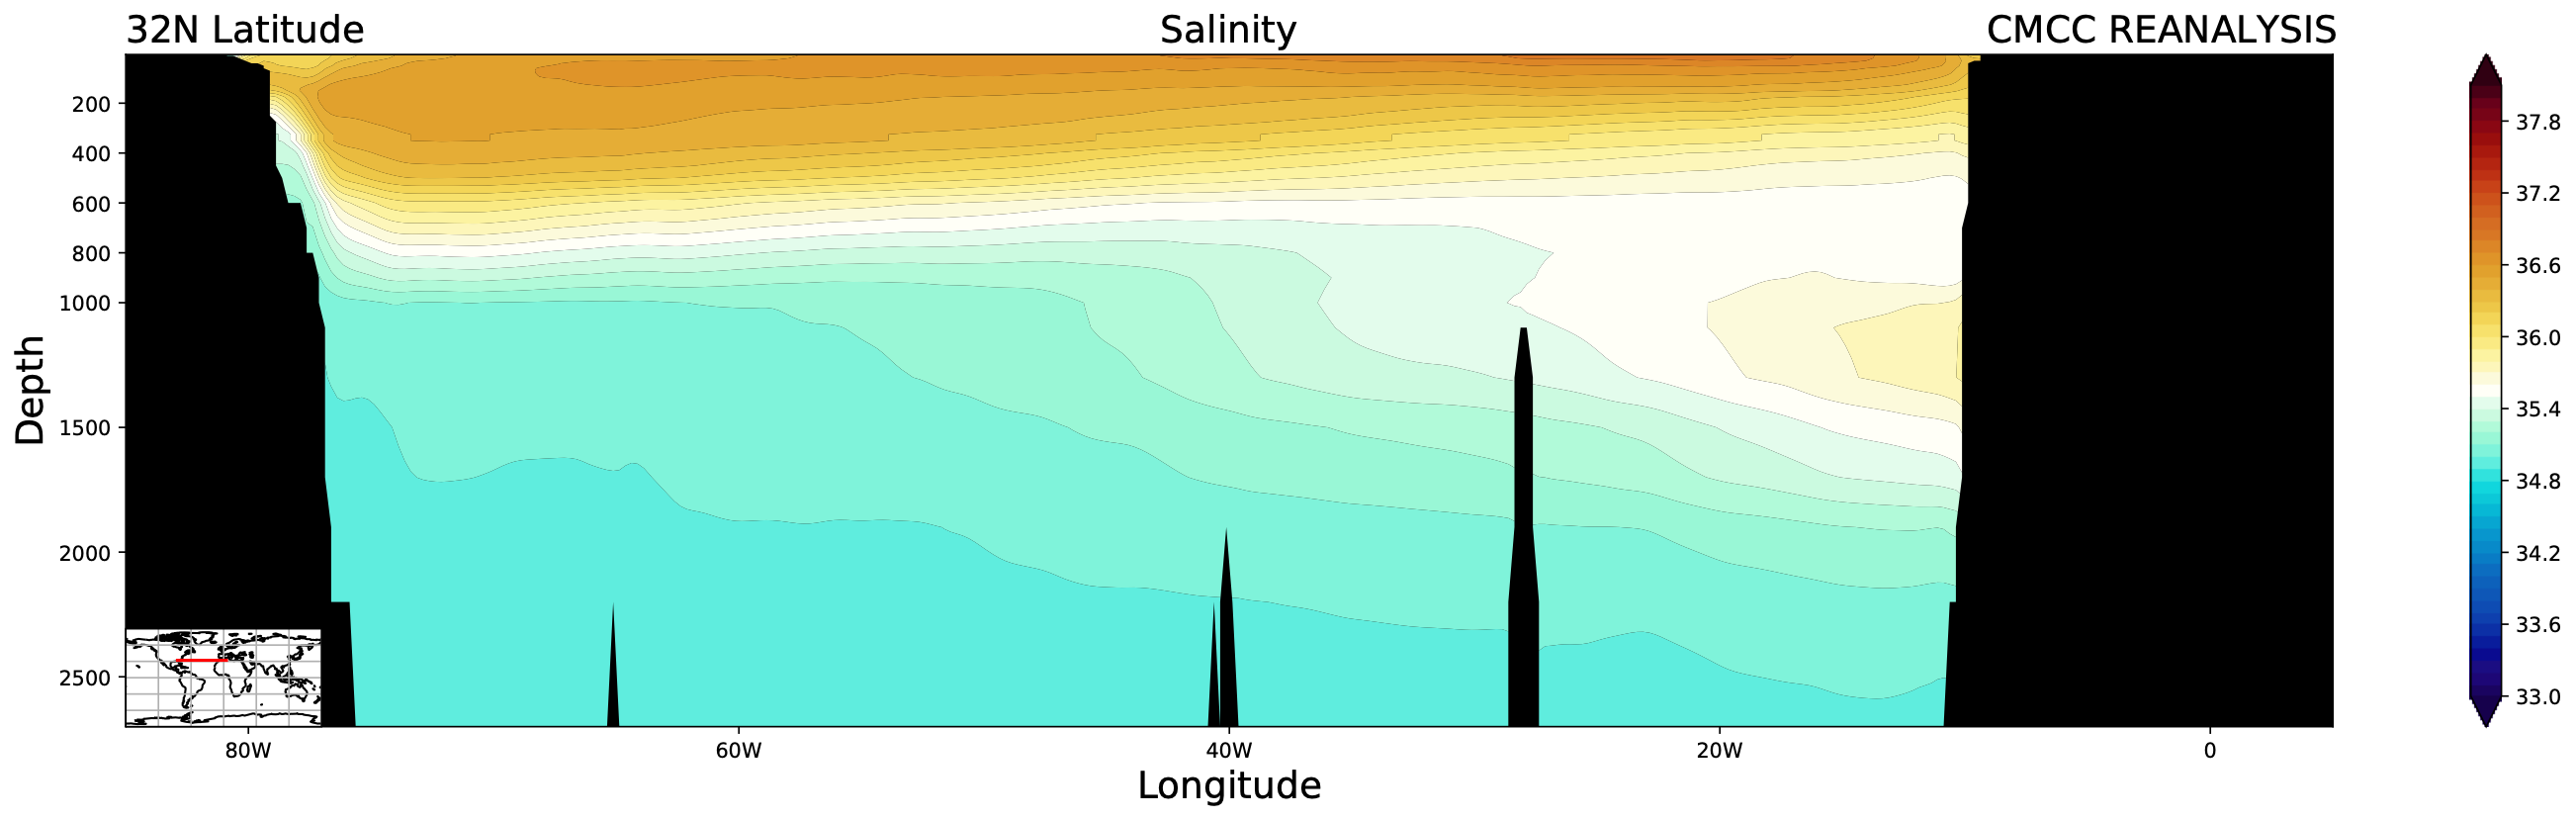
\includegraphics[width=0.5\linewidth]{upload/32image.png}
	\caption{The vertical structure of the Pacific Ocean}
	\label{fig:fig7}
\end{figure}


The vertical structure of the Pacific Ocean (Figure \ref{fig:fig7}) is
different and what we see is a situation where salinity is slowly
varying getting fresher toward the surface, with the thin saline water
in the subtropics a clear signature of the equatorial upwelling and the
Antarctic water filling the abyssal plains. The Indian Ocean is similar
to the Pacific South of the Equator but North of the Equator at this
longitude is fresher.

\begin{figure}[htpb!]
	\centering
	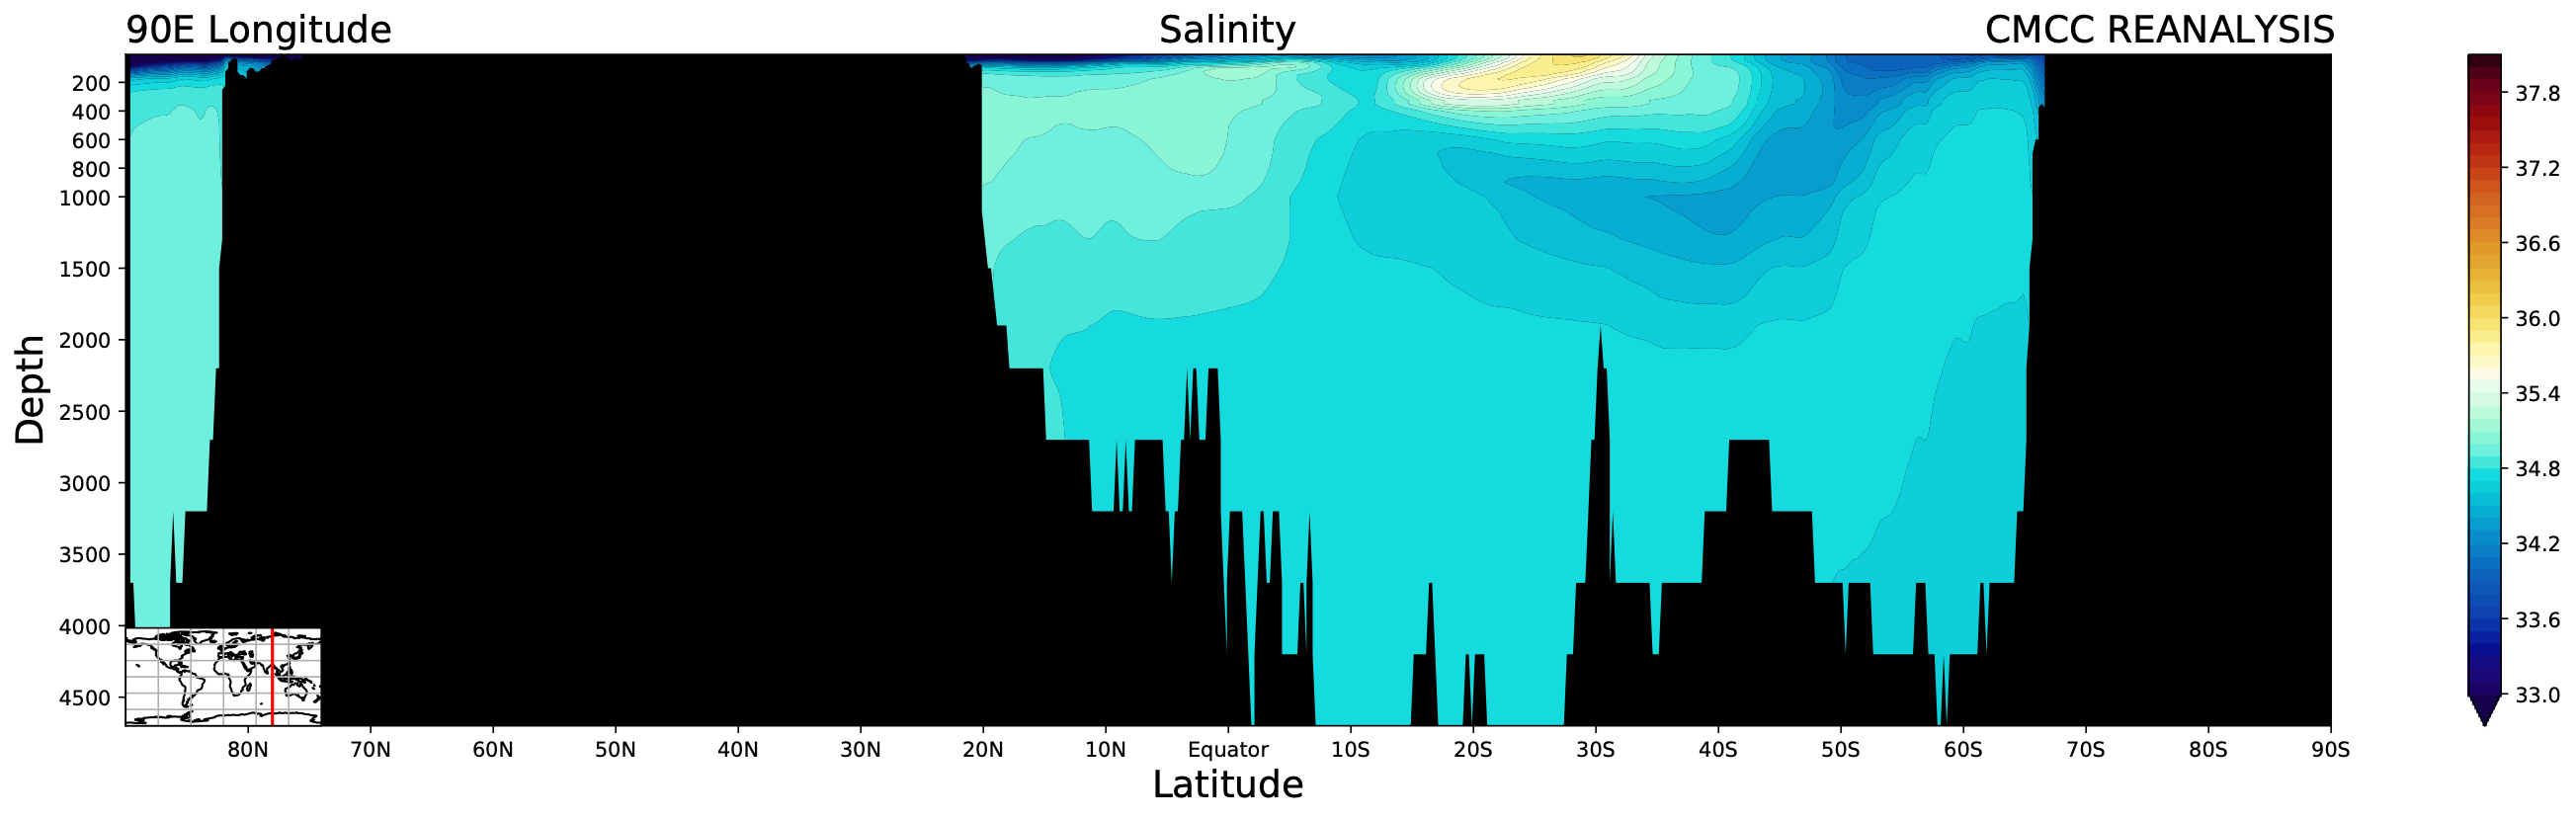
\includegraphics[width = 0.4 \textwidth]{upload/33image.png}
	\caption{As in Fig. \ref{fig:fig7} but for 90E longitude}
	\label{fig: fig8}
\end{figure}

The Indian Ocean (Figure \ref{fig: fig8}) shown here as a section
cutting essentially through the Bay of Bengal, shows a similar strong
stratification, but there are only weak signs of an equatorial upwelling
of cold water.



We can gain more insights in the equatorial structure by looking at a
longitudinal section along the Equator in the Pacific (Figure \ref{fig:fig9}). Here we see the general difference between the
Atlantic and the Pacific, but we also see that the salinity is following
the slant of the equatorial thermocline and the equatorial upwelling in
the East Pacific. The effect of the major precipitation center of ITCZ
in the West Pacific is visible in fresh water at the surface in the
West.

\subsection{Influence of the ocean}

\paragraph{The continentality effect}
It makes continental summers warmer and winters cooler than the adjacent ocean areas. The oceans have this effect because of their large heat storage capacity and because part of  the energy that they retain from solar input during the summer they return to the atmosphere in the forms of sensible and latent heat and longwave radiation the following winter. Conversely, the continents have the reverse effect, strengthening the seasonal temperature contrasts

\paragraph{Ocean currents}
They can transport heat from low to high latitudes. (in the Gulf Stream of the North Atlantic). This contributes to much higher winter air temperatures over mid-to-high latitude oceans than over adjacent land areas at the same latitude.

\paragraph{The overall basin
	circulation}\label{the-overall-basin-circulation}

The surface currents of the Atlantic ocean are shown in Figure \ref{fig:fig10}. As we might have suspected from the temperature coast that reaches all the way across the North Atlantic to Europe, the Gulf Stream. Strong currents are also visible in the Equatorial area
where they connect to the mid-latitude circulation forming a large circular system, the Subtropical Gyre. The South Atlantic has a similar gyre in the subtropical region, but at higher latitudes we can notice a strong westerly current cutting all along the basin, essentially along a latitude line between 40S and 50S.

\begin{figure}[htpb]
	\centering
	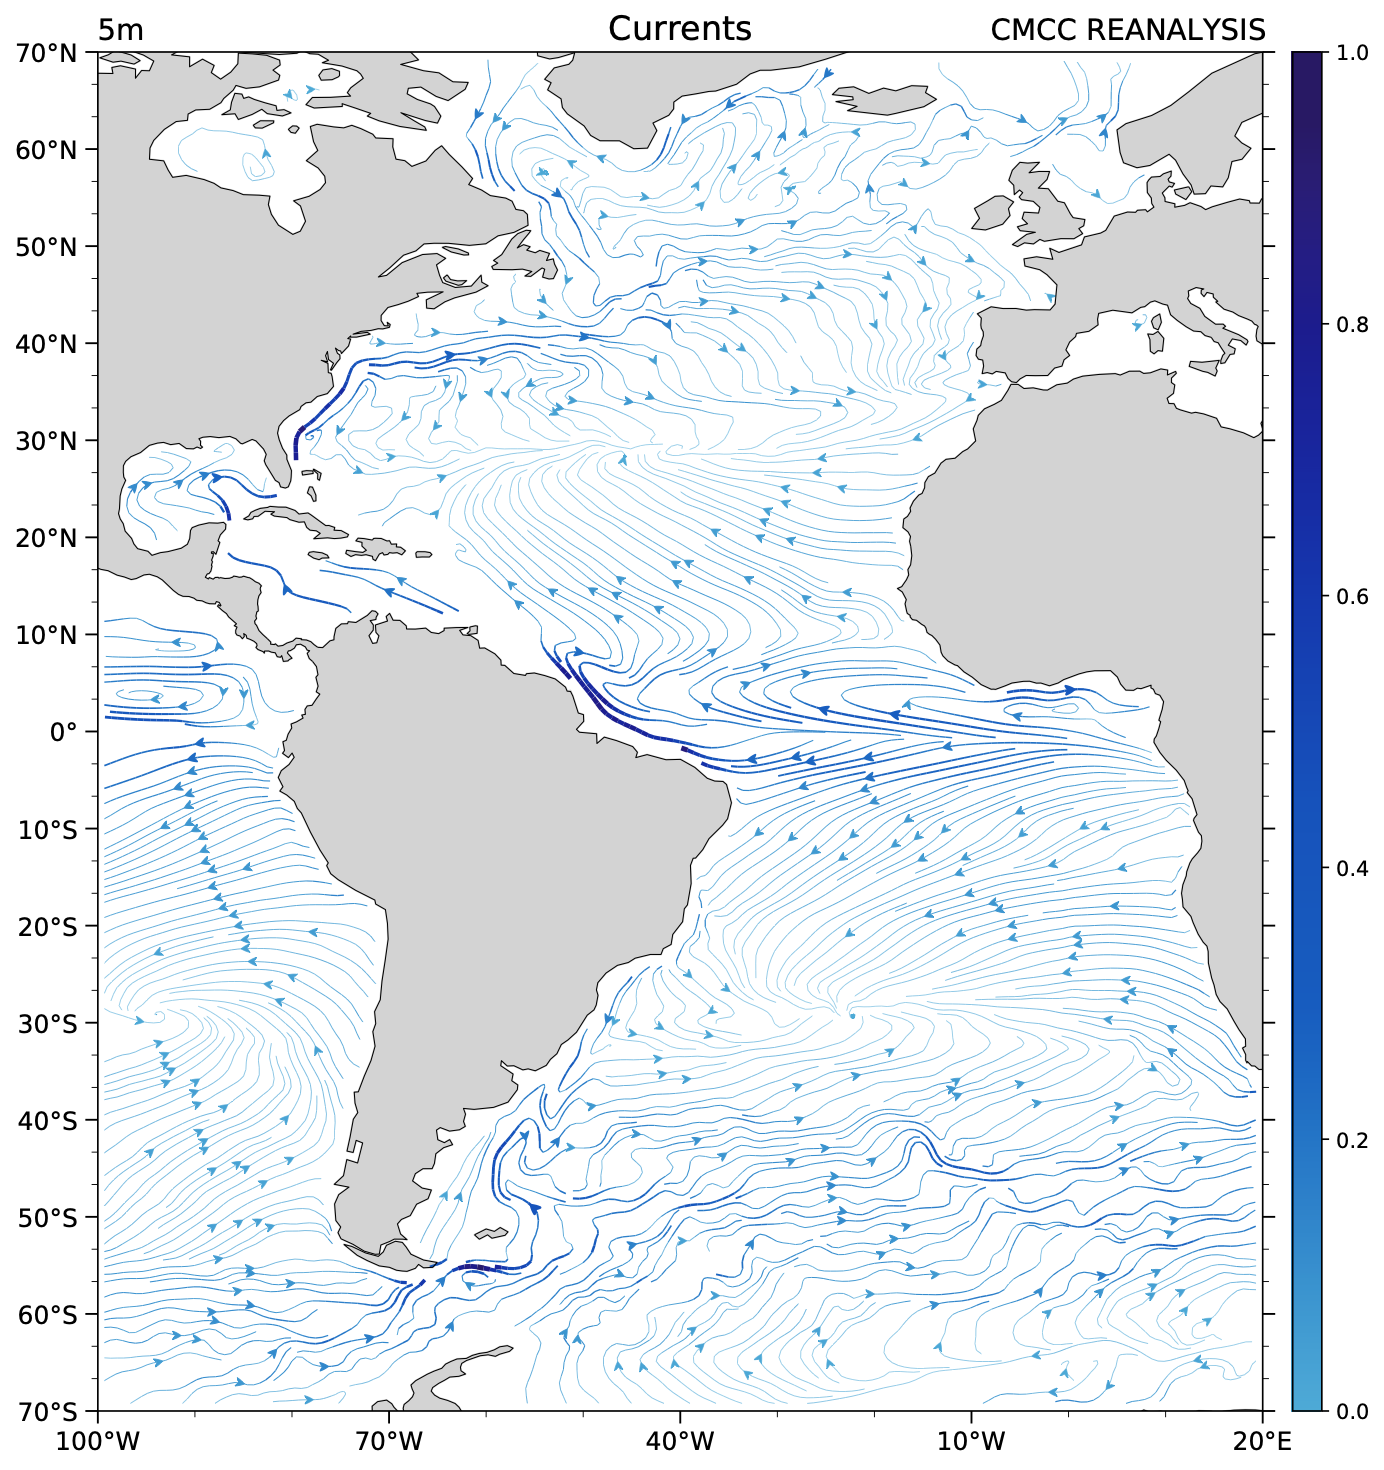
\includegraphics[width = 0.4 \textwidth]{upload/35image.png}
	\caption{The surface currents of the Atlantic ocean} \label{fig:fig10}
\end{figure}

The North Pacific surface circulation is shown in Figure \ref{fig:fig11}. We can notice here again a strong current along the Western boundary of the basin that than feed into a basin wide gyre that connects to the equatorial circulation. The boundary current, known her as the Kuroshio Current, is very narrow and intense along the Japan coast, as it is also the case of the Gulf Stream in the Atlantic, and it tapers into a wide system of streams and eddies into the open ocean.

It is possible to see also local system, like the small gyre off the Alaskan coast and similar circulation in the marginal seas, like the Sea of Okhotsk, near the Siberian coast. Their presence is remarkable as we are looking here at climatological averages over more than 40 years and so they are stable and persistent features. This is another reminder of how even relatively smaller feature in the ocean can be climatologically persistent over many years.

\begin{figure}[htpb]
	\centering
	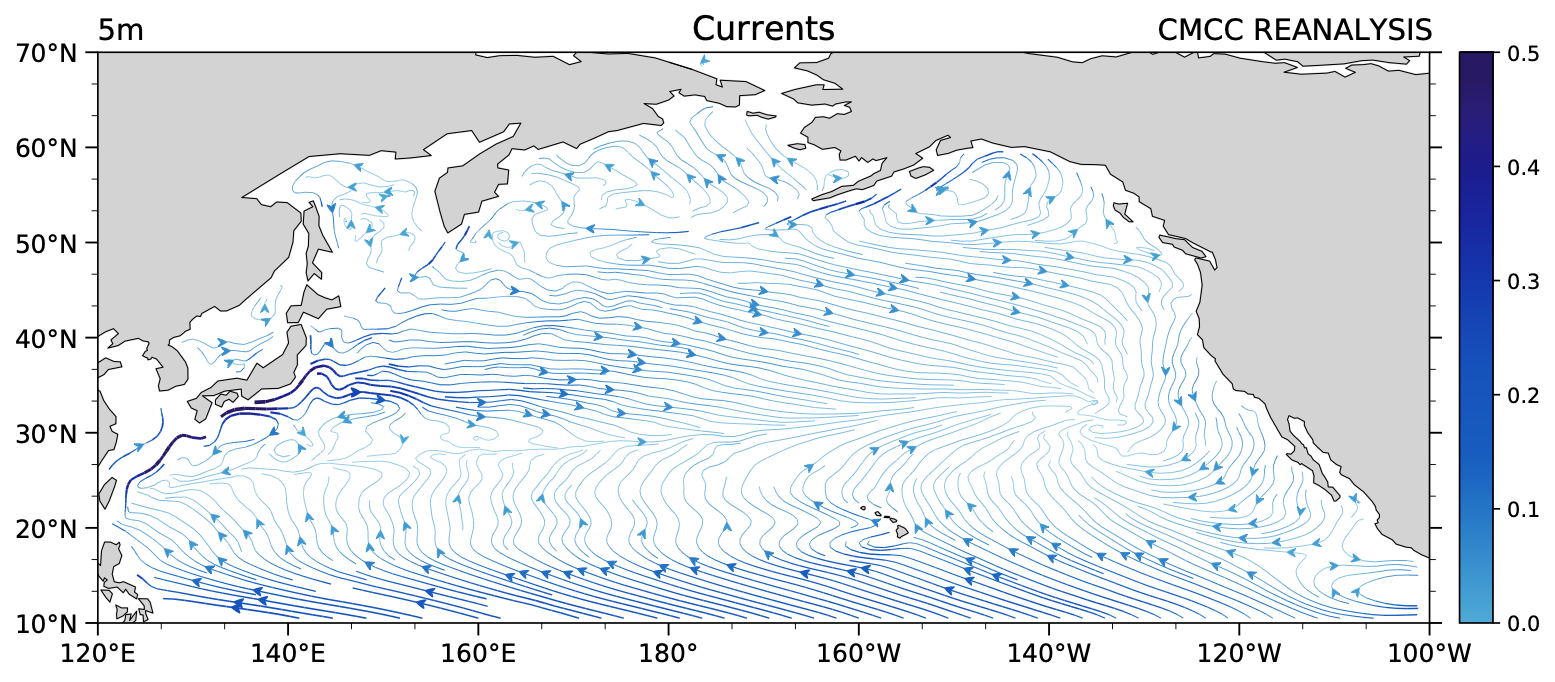
\includegraphics[width = 0.4 \textwidth]{upload/i36mage.png}
	\caption{The North Pacific surface circulation} \label{fig:fig11}
\end{figure}

The circulation of the South Pacific Ocean is shown in Figure \ref{fig:fig12}. The subtropical gyre is visible also here, but there is a weak indication of a western intensification current in the West pacific, close to the coasts of Australia and New Zealand. The strong high latitude current that we have seen in the Atlantic is also present here end evidently connect to the other basin through the Drake Passage, that is the Straits between South America and Antarctica.

\begin{figure}[htpb]
	\centering
	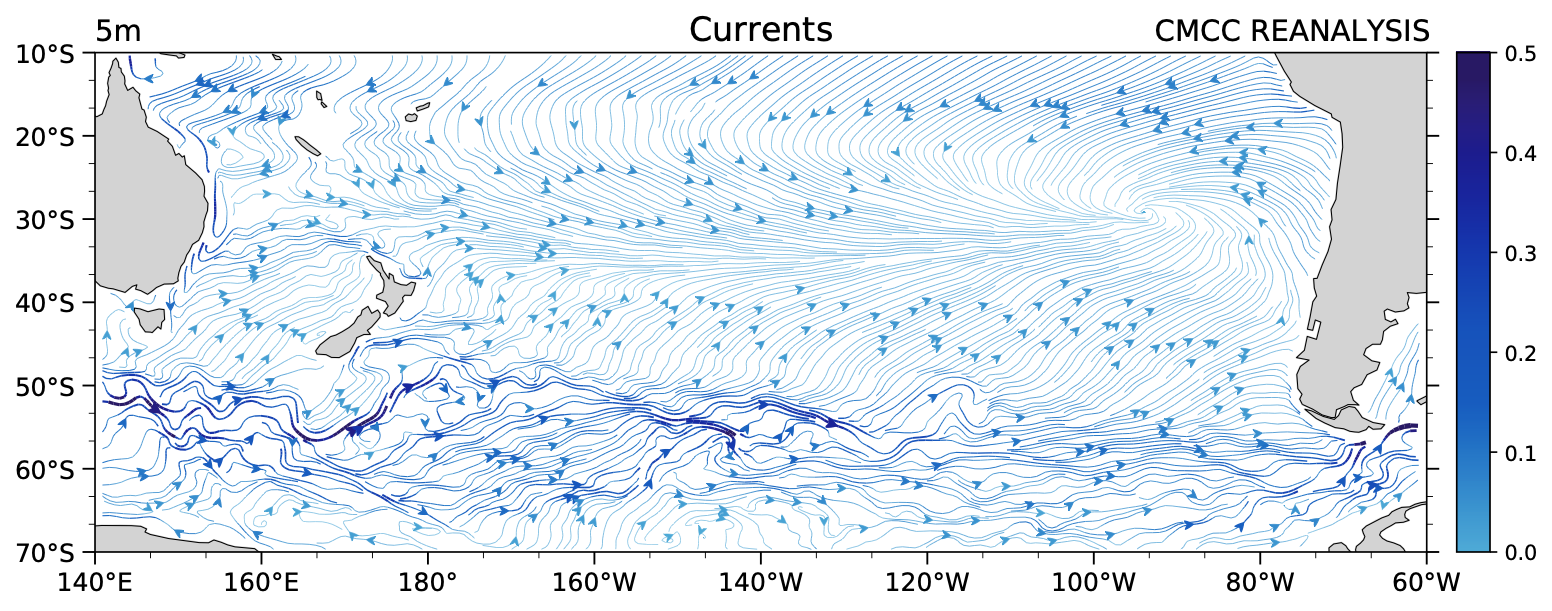
\includegraphics[width = 0.5 \textwidth]{upload/37image.png}
	\caption{The circulation of the South Pacific Ocean} \label{fig:fig12}
\end{figure}

The Indian Ocean circulation is shown in Figure \ref{fig:fig13}. The Indian Ocean is confined by continental masses in the north, so it is mostly composed of the equatorial region and the midlatitudes are all in the Southern Hemisphere. The subtropical gyre is present, together with features North of Madagascar. A boundary current develops on the African coast, The westerly current in the southern mid-latitudes is visible also here, strong and with a vigorous eddy field.

\begin{figure}[htpb]
	\centering
	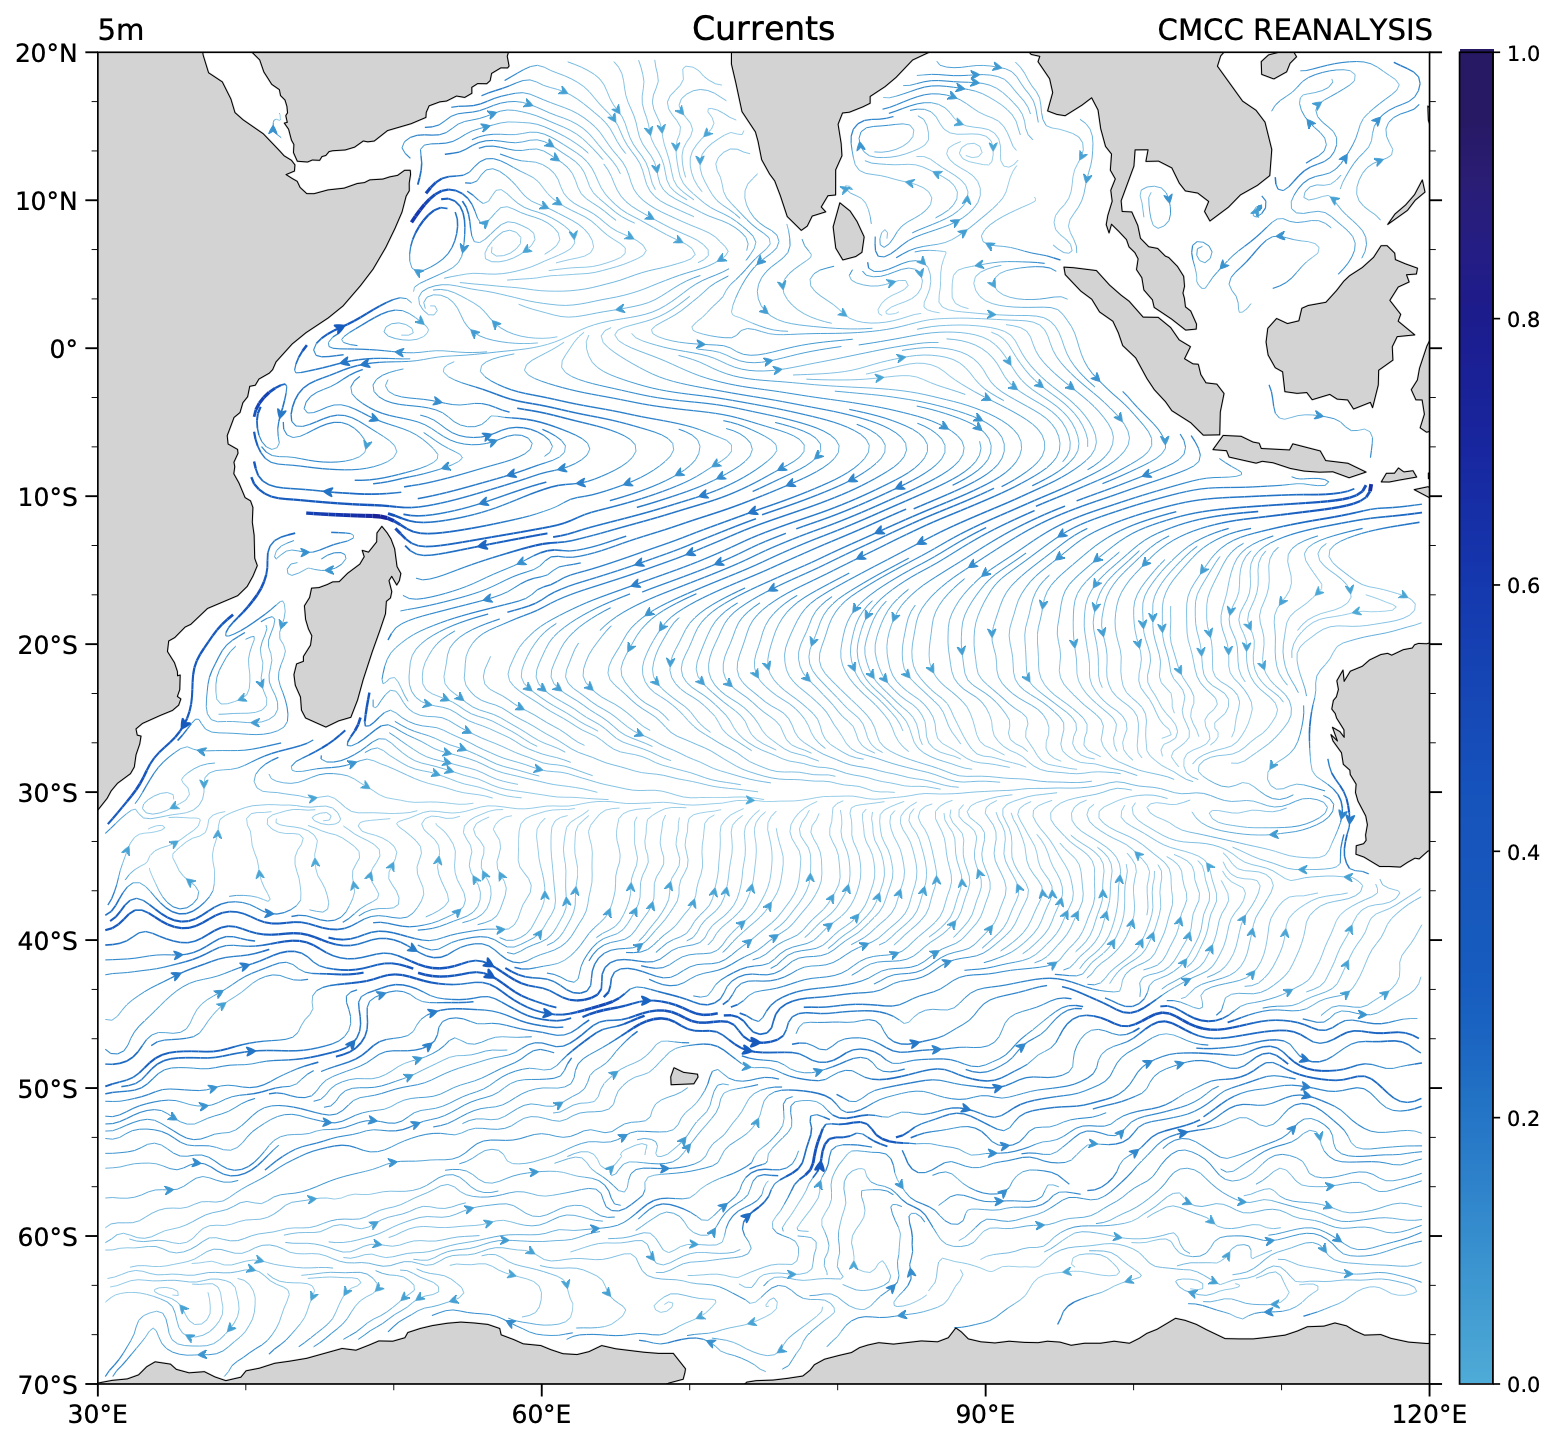
\includegraphics[width = 0.35\textwidth]{upload/38image.png}
	\caption{The Indian Ocean circulation} \label{fig:fig13}
\end{figure}

At this point we can suspect that there is probably a continuous ring of currents around Antarctica and this can be confirmed by the bottom panel of Figure \ref{fig:fig13}  that shows the entire extent around a
longitude circle of the current, known as the Antarctic Circumpolar
Current. It is a strong, highly turbulent system that connects all the
Ocean Basins.
\\

\subparagraph{The equatorial
	circulation}

The Equator is a special place for the atmosphere and so it is a special
place also for the Oceans. The circulation in this area is strongly
coupled with the atmospheric circulation and it is often characterized
by both westerly and easterly currents and by special behaviours right
at the Equator line. Futhermore, it is also very different from ocean to
ocean.

The equatorial current system in the Pacific Ocean is shown in Figure \ref{fig:fig14}. It is a complex system composed of two easterly
currents, the North and South Equatorial currents, sandwiching the
westerly Equatorial countercurrent. It is possible to notice that at the
Equator the currents are strongly easterly and diverging, leading to the
emergence of upwelling at the Equator by Ekman transport.

\begin{figure}[htpb]
	\centering
	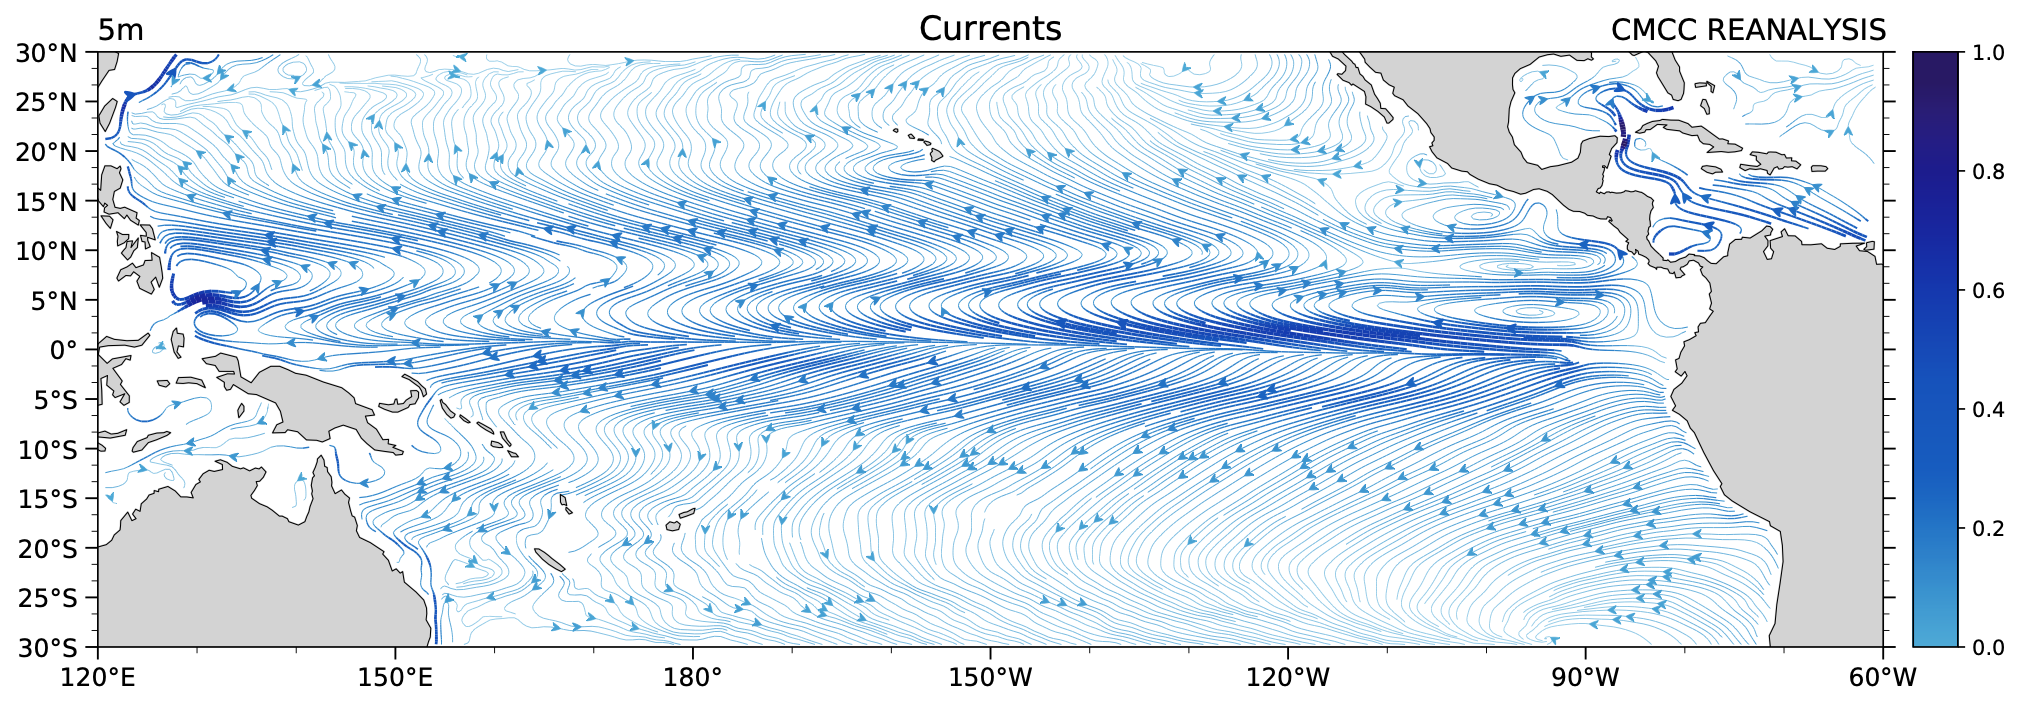
\includegraphics[width = 0.4 \textwidth]{upload/39image.png}
	\caption{The equatorial current system in the Pacific Ocean} \label{fig:fig14}
\end{figure}

The complexity of the equatorial current system can be further
appreciated by looking at the vertical section of the zonal current at
the Equator. A strong westerly current below the
surface, slanting from the West Pacific to the East Pacific, is visible
at depth between 200 and 300m. The speed is in excess of 1 m/s and it
gets progressively shallower in the East.

It is however part of an alternation of westerly and easterly currents
that become progressively weaker as they get deeper. They are centered
almost perfectly at the Equator, as it can be seen in Figure \ref{fig:fig16}. The latitudinal position of the undercurrent is very tightly controlled by rotational effects and it precisely tracks the position of the equatorial line.

\begin{figure}[htpb]
	\centering
	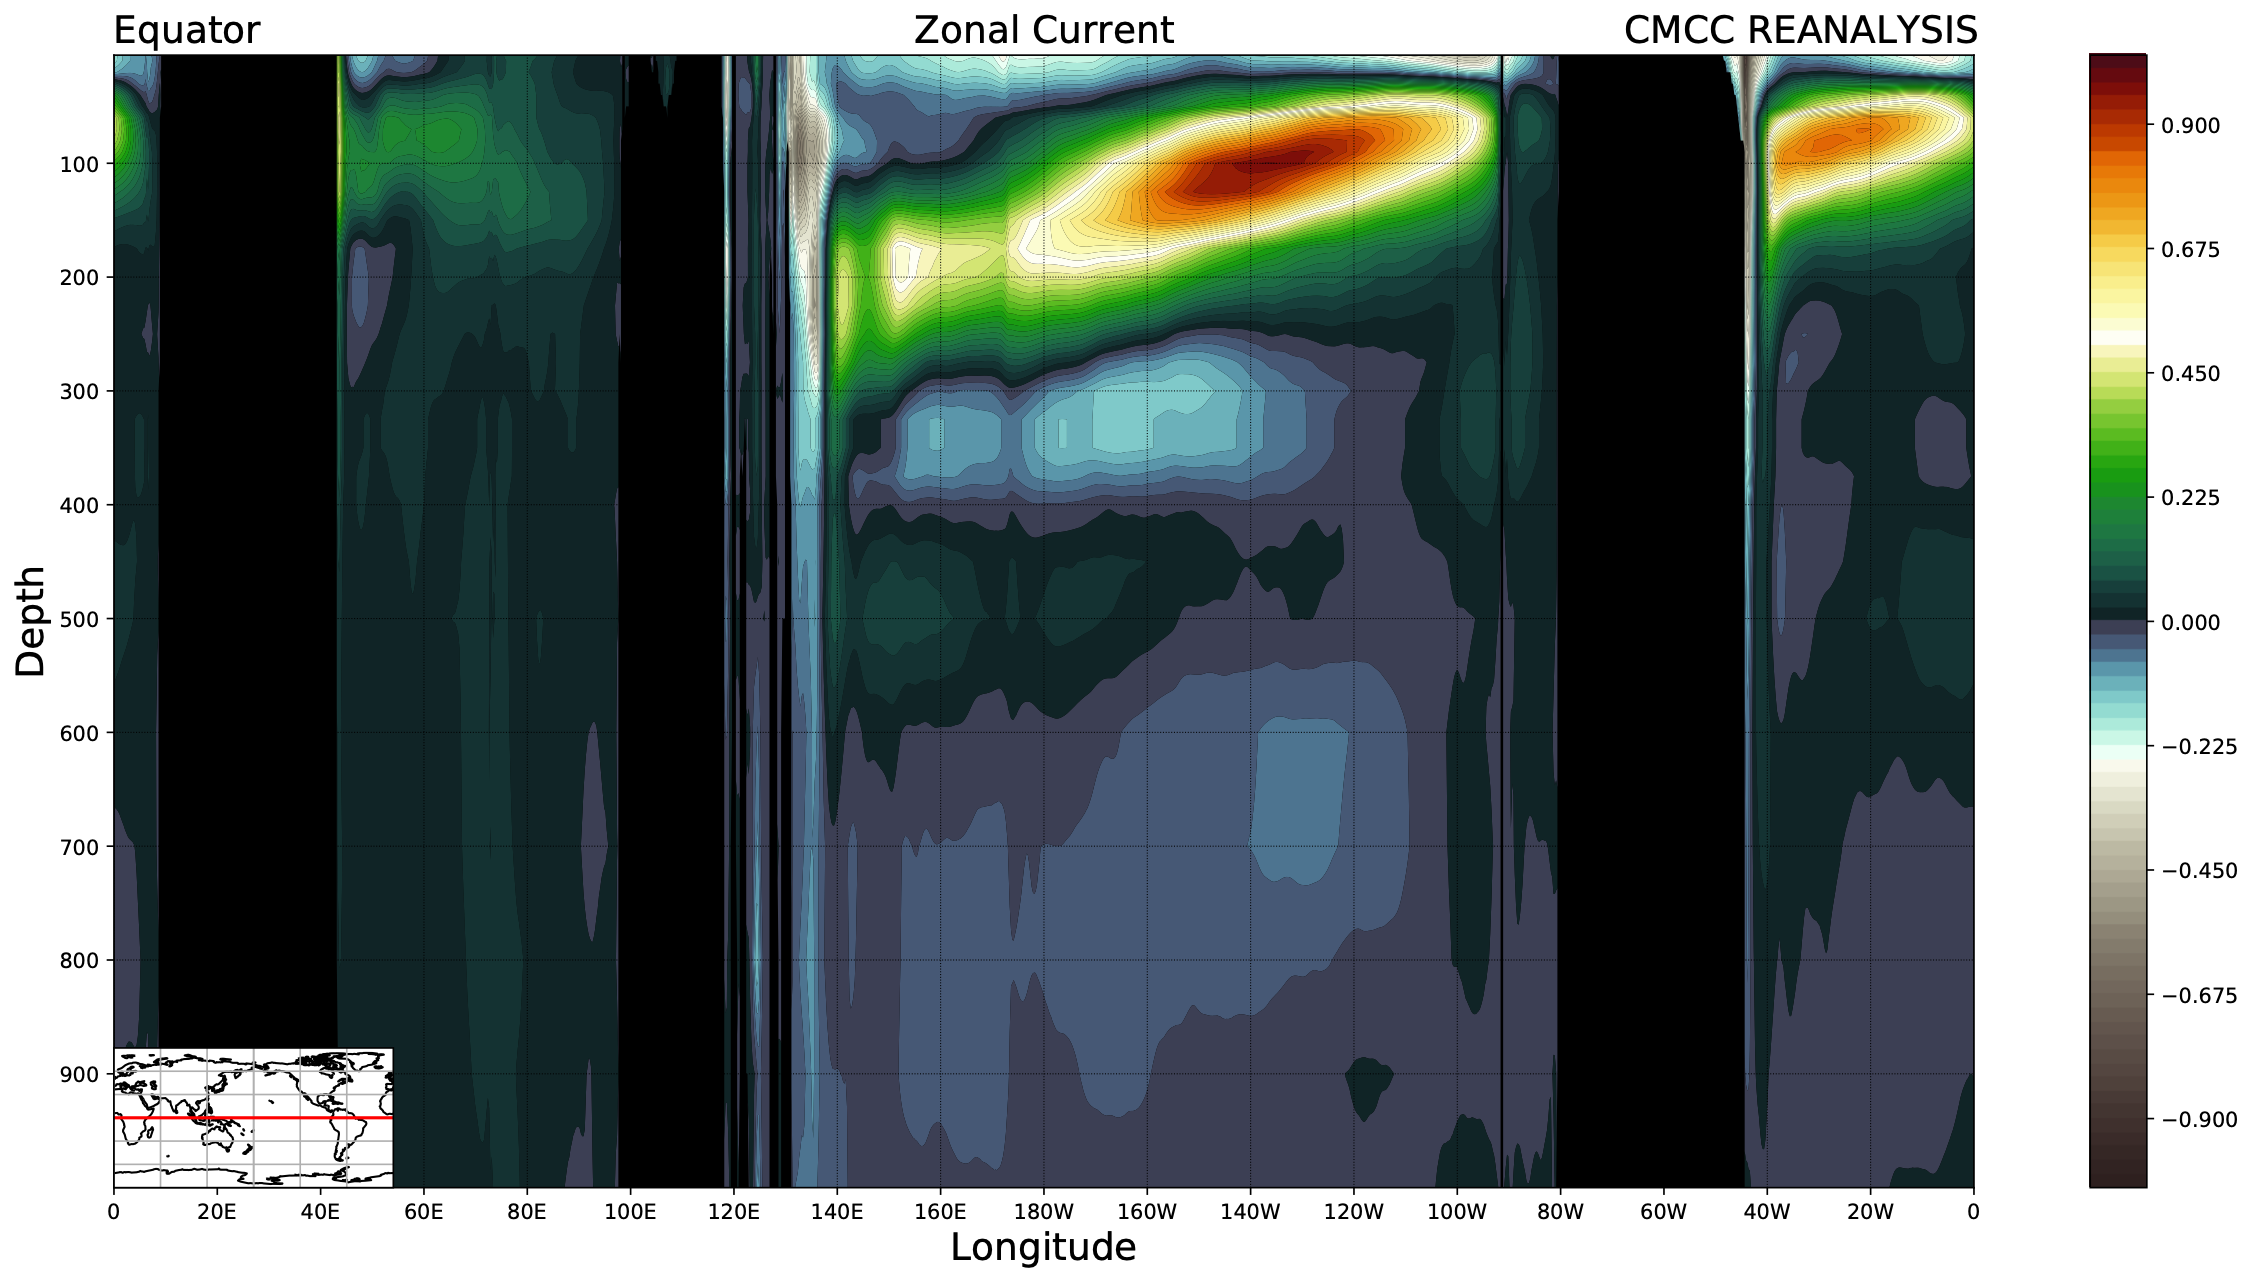
\includegraphics[width = 0.4 \textwidth]{upload/40image.png}
	\caption{Alternation of westerly and easterly currents} \label{fig:fig16}
\end{figure}

The equatorial Atlantic Ocean surface circulation (Figure 1.14). It is possible to see the easterly South Equatorial
Current that is straddling the Equator between 5S and 5N. The North
equatorial Countercurrent is westerly and it covers the area between 5N
and 10N, and the weaker North Equatorial Current is located at northern
latitudes. The equatorial flow is divergent and also in this case we can
presume the existence of upwelling at the Equator. A strong coastal
current is visible as the Guinea Current, in the Gulf of Guinea. The
South Equatorial Current feeds into the North Brazilian Current that
then flows northward along the South America coast, taking different
names as it finally emerges as the Caribbean Current in the Caribbean
sea.
\begin{figure}[htpb!]
	\centering
	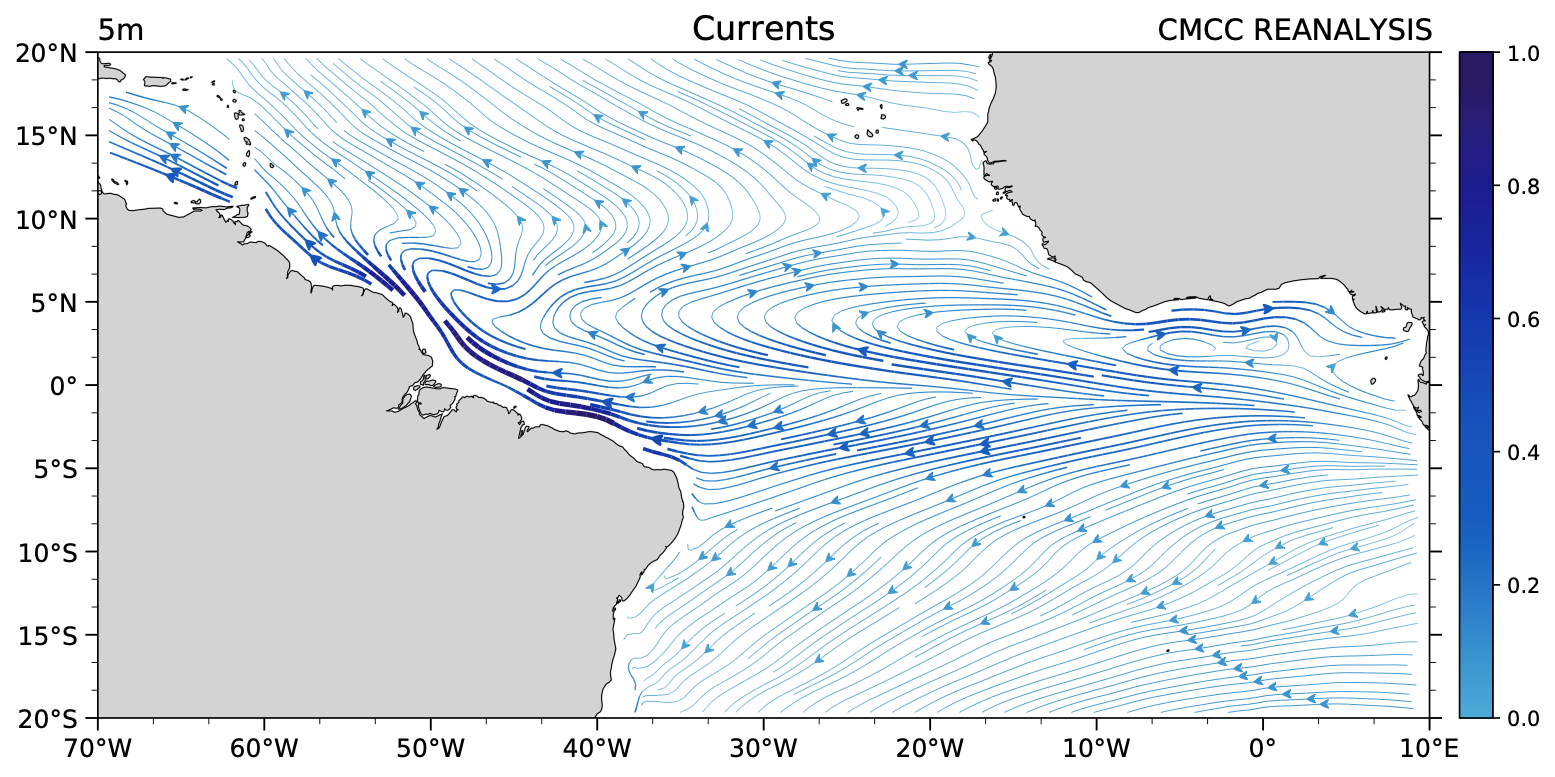
\includegraphics[width=0.45\linewidth]{upload/41image.png}\quad 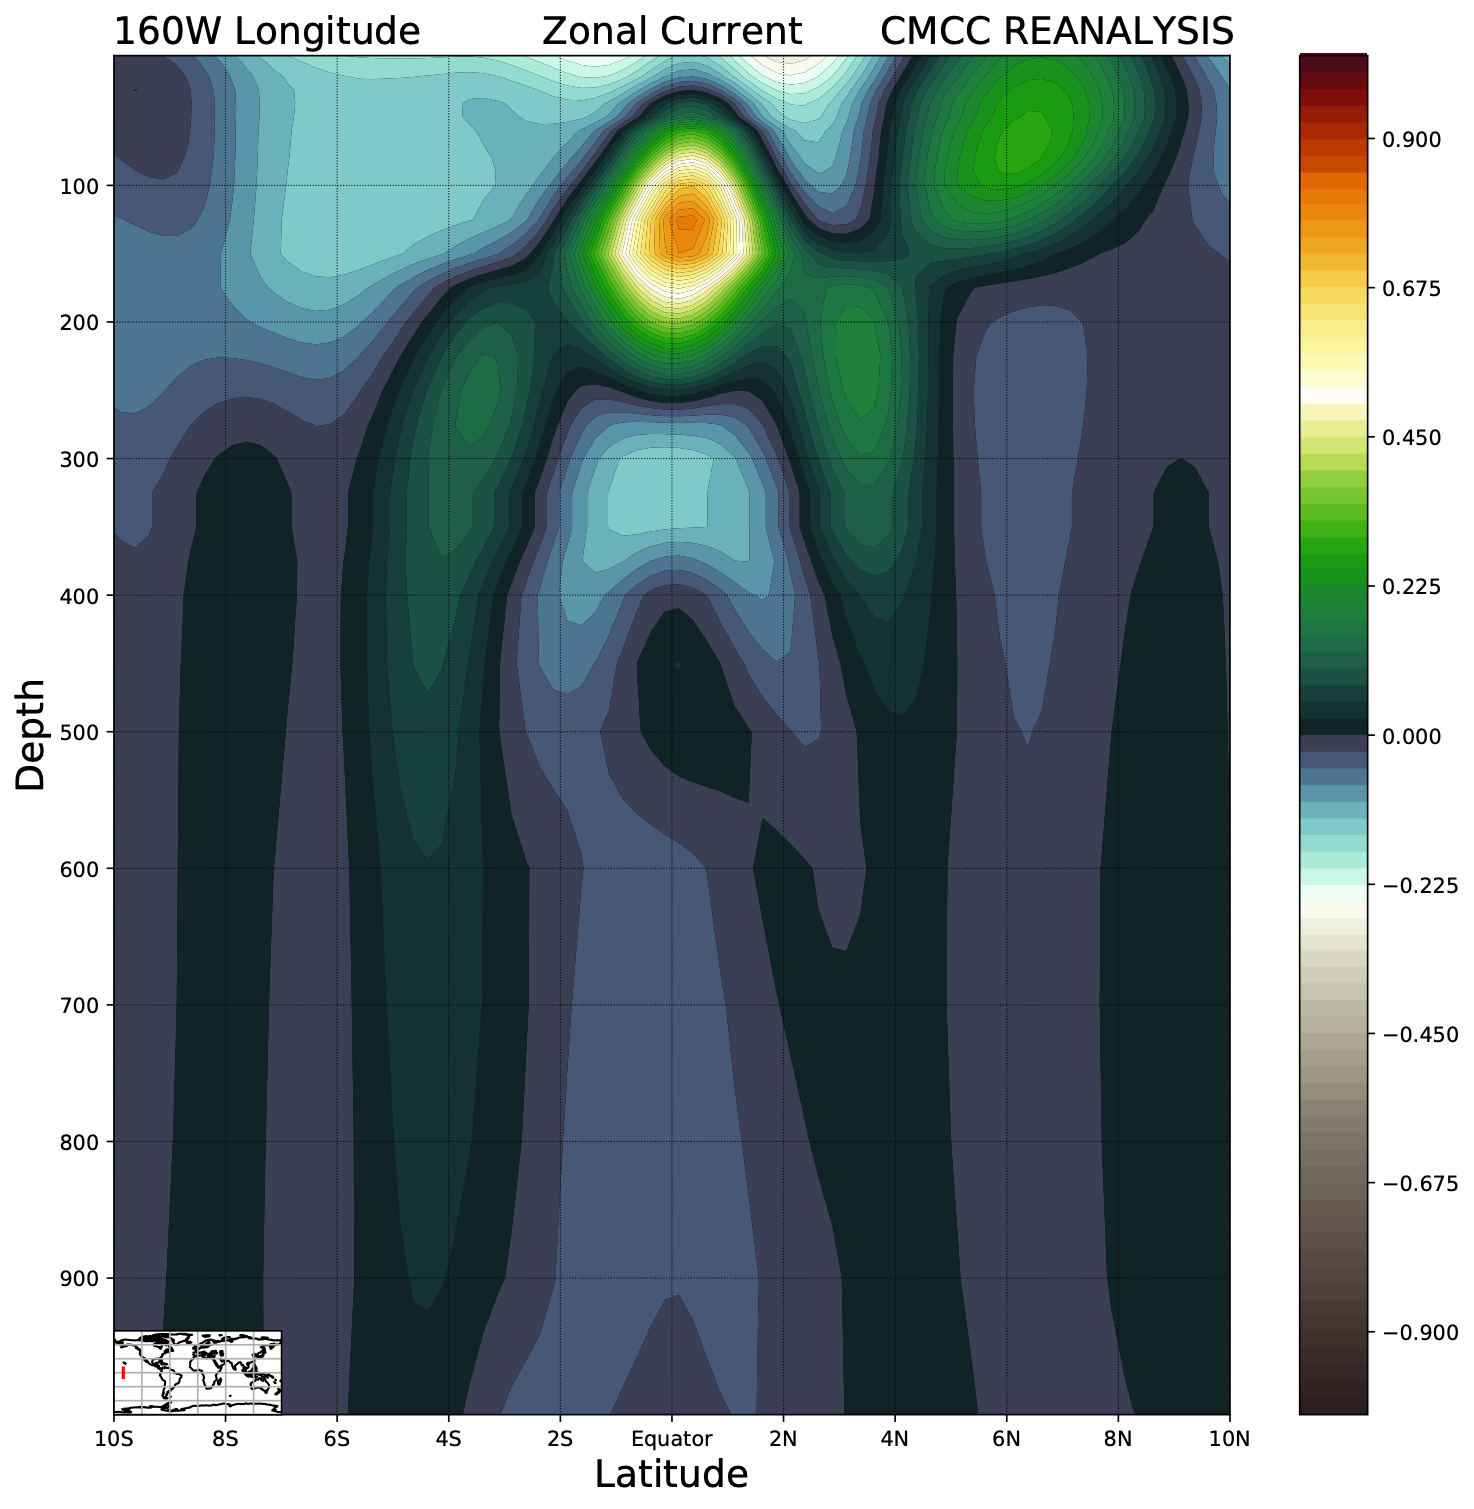
\includegraphics[width=0.3\linewidth]{upload/42.png}
	\caption{The equatorial Atlantic Ocean surface circulation and the structure of currents and undercurrents}
	\label{fig:fig17}
\end{figure}
A similar structure of alternating westerly and easterly undercurrents
exist also in the equatorial Atlantic (Figure 1.14), but it
is weaker and only the first westerly maximum is well visible. It is
also slanting towards the East, but the maximum is reached more towards
the western boundary of the basin with respect to the Pacific Ocean. The
deeper easterly jets are also much less weaker. The undercurrents jets
are essentially absent in the Indian Ocean.


\paragraph{The Gulf Stream}\label{the-gulf-stream}

The current system of the Gulf Stream is one of the major feature of the
global ocean circulation.


\subparagraph{The Kuroshio}\label{the-kuroshio}

The current system of the Kuroshio is one of the major features of the
global ocean circulation.


\begin{figure}[htpb!]
	\centering
	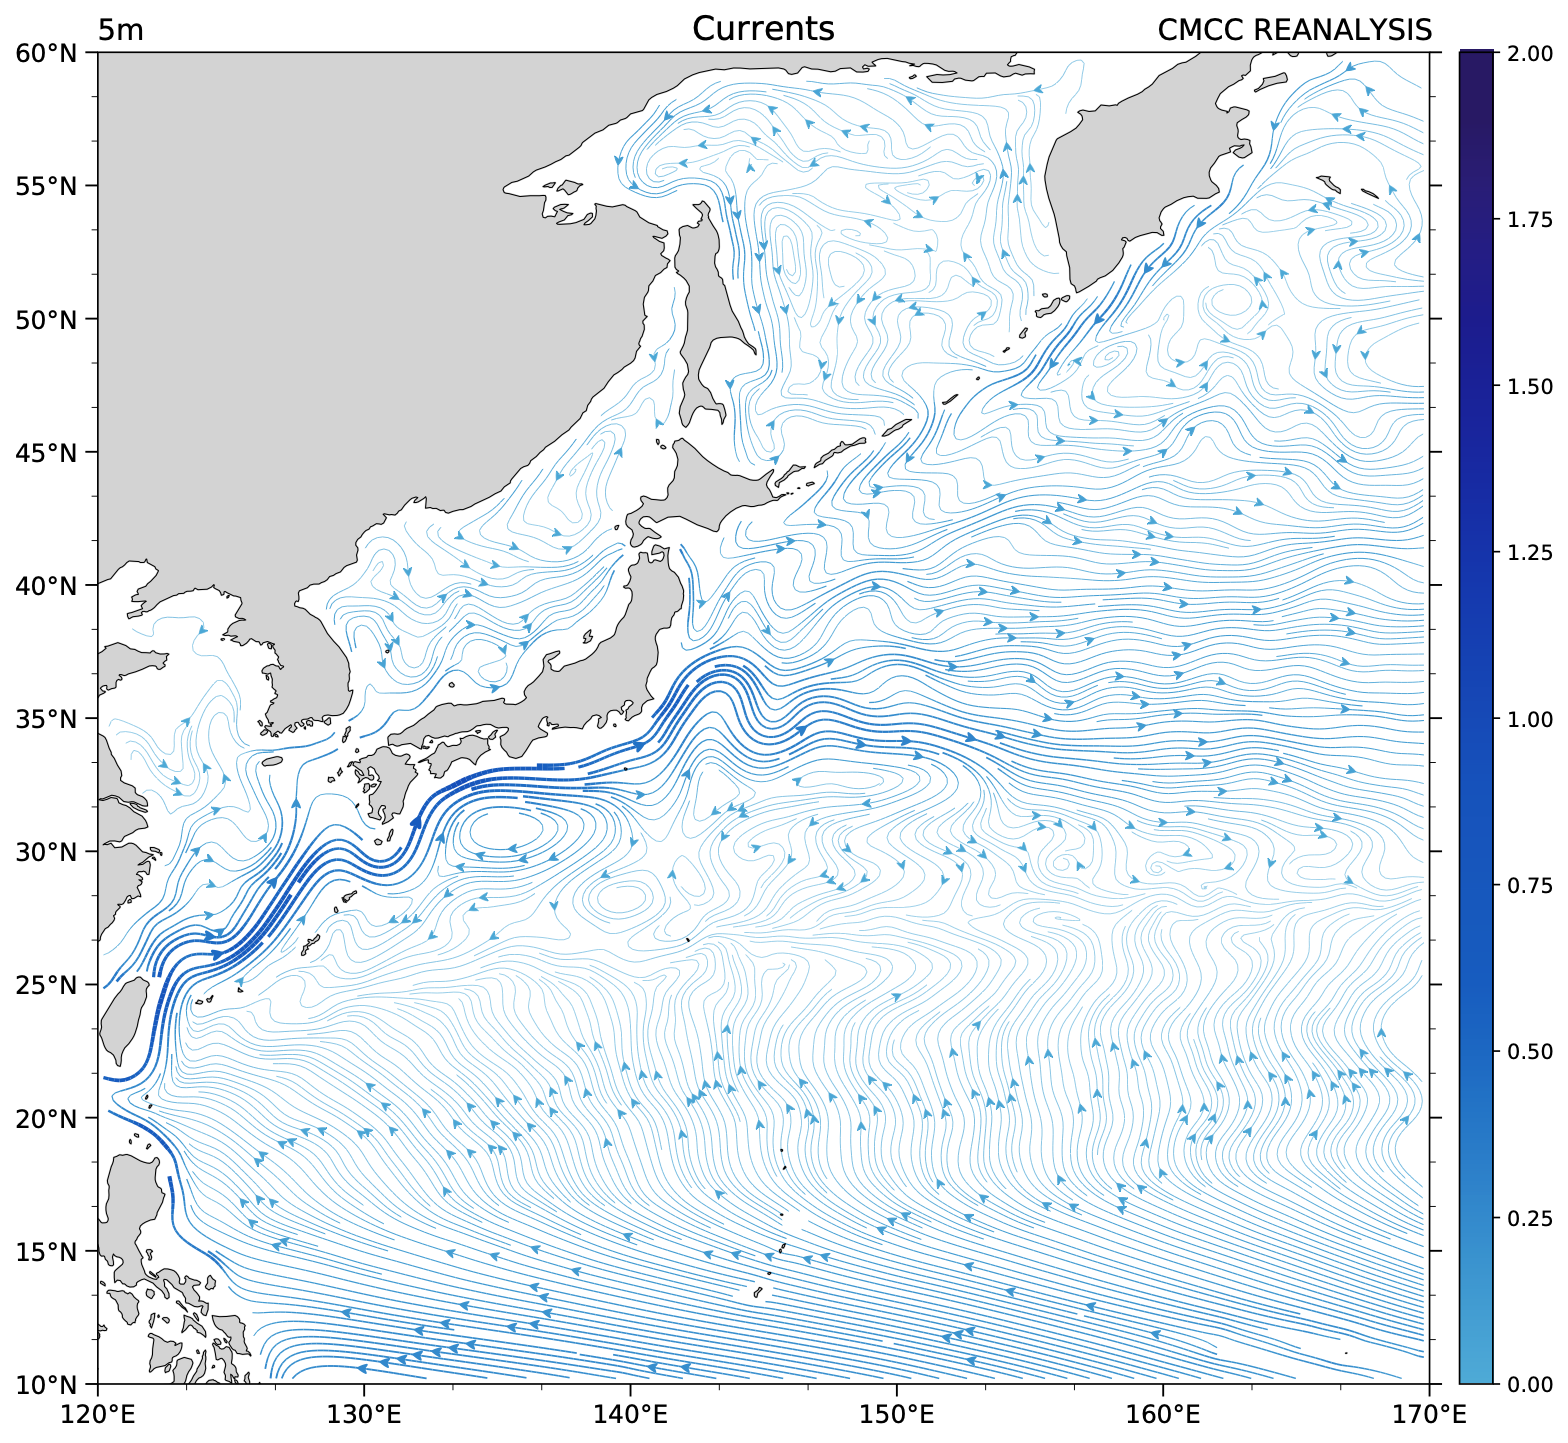
\includegraphics[width = 0.30 \textwidth]{upload/44.png}\quad 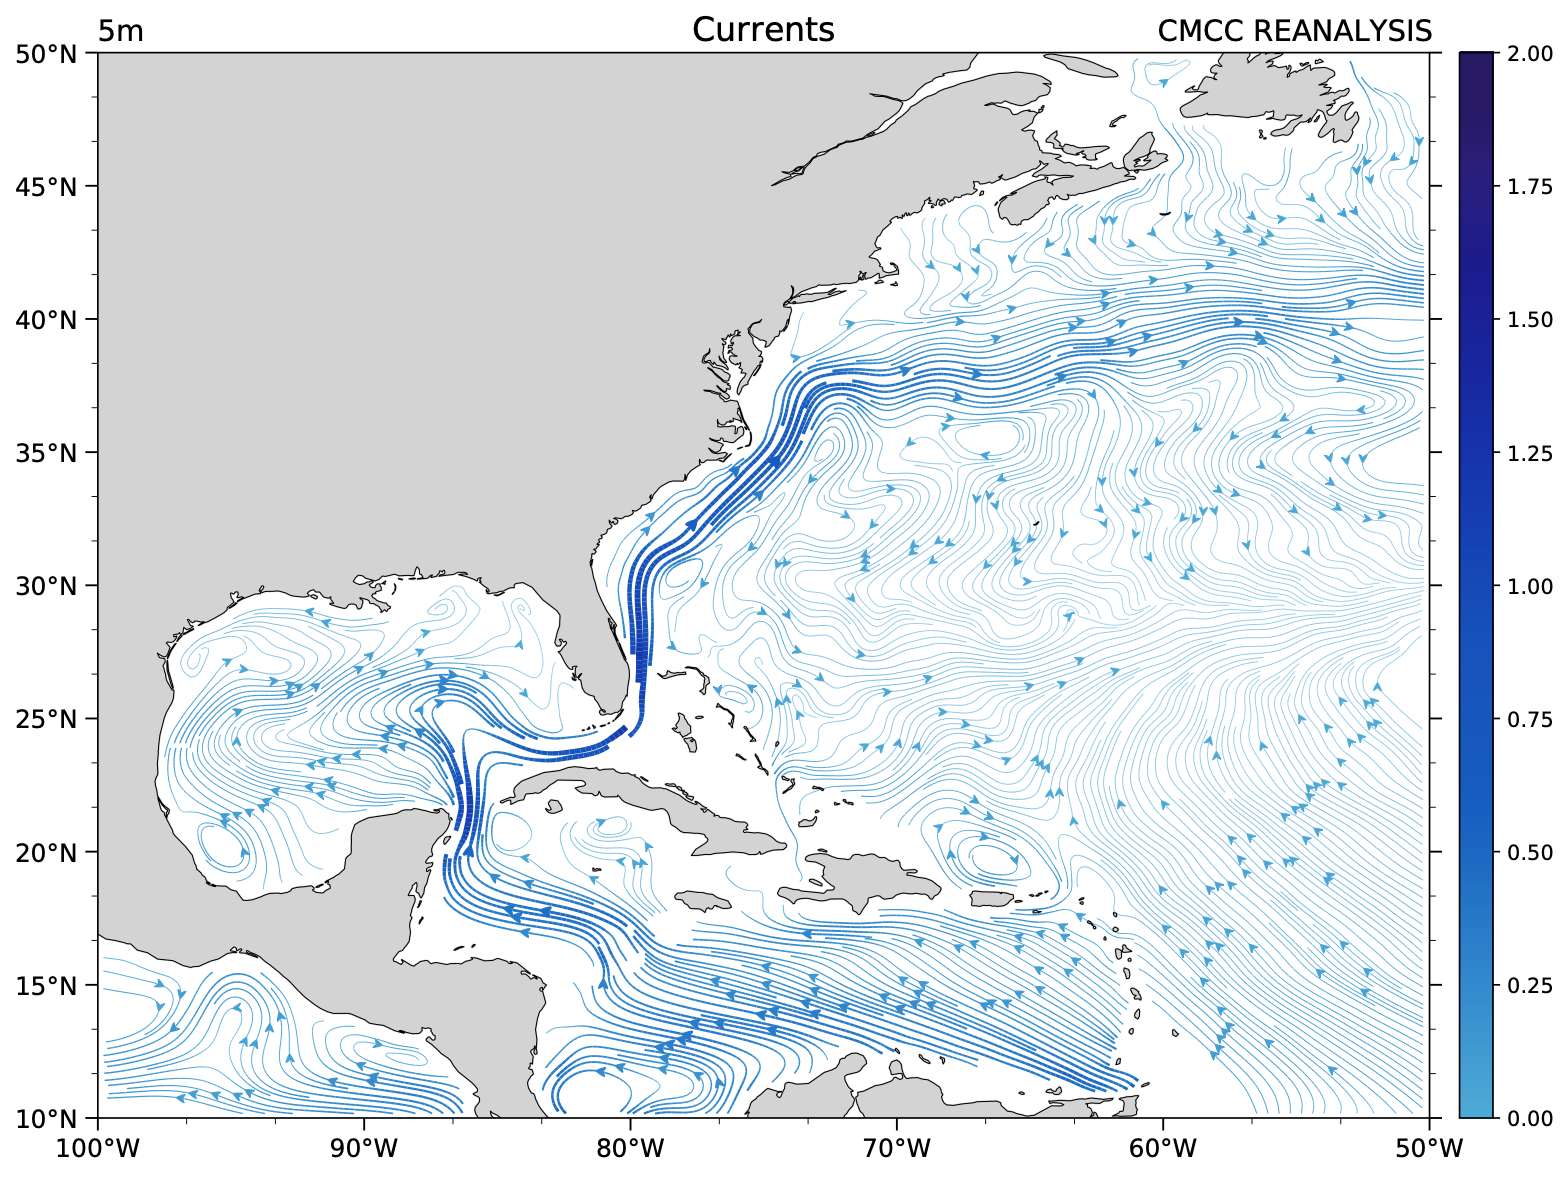
\includegraphics[width = 0.35\textwidth]{upload/43.png}
	\caption{The Kuroshio on the left and Gulf Stream on the right} \label{fig:}
\end{figure}

\begin{figure}[htpb!]
	\centering
	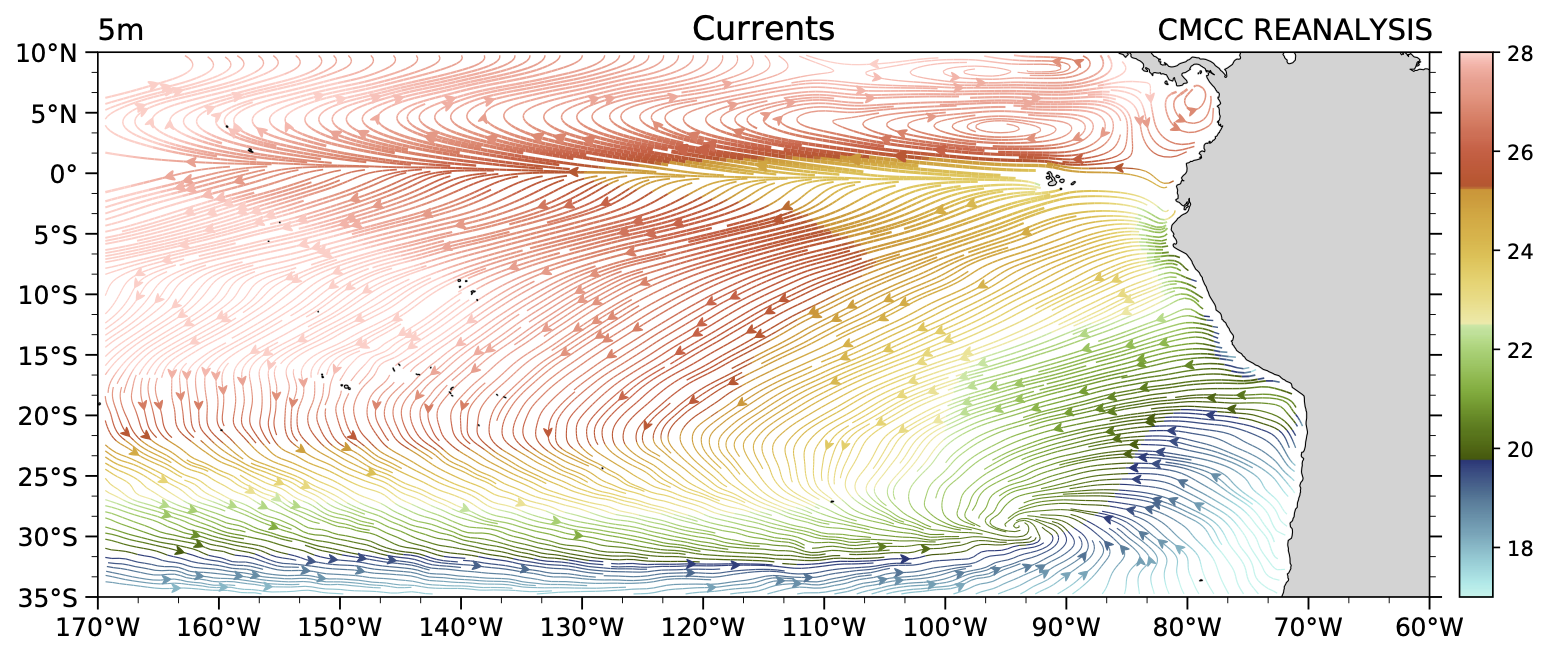
\includegraphics[width = 0.45 \textwidth]{upload/45.png}\quad 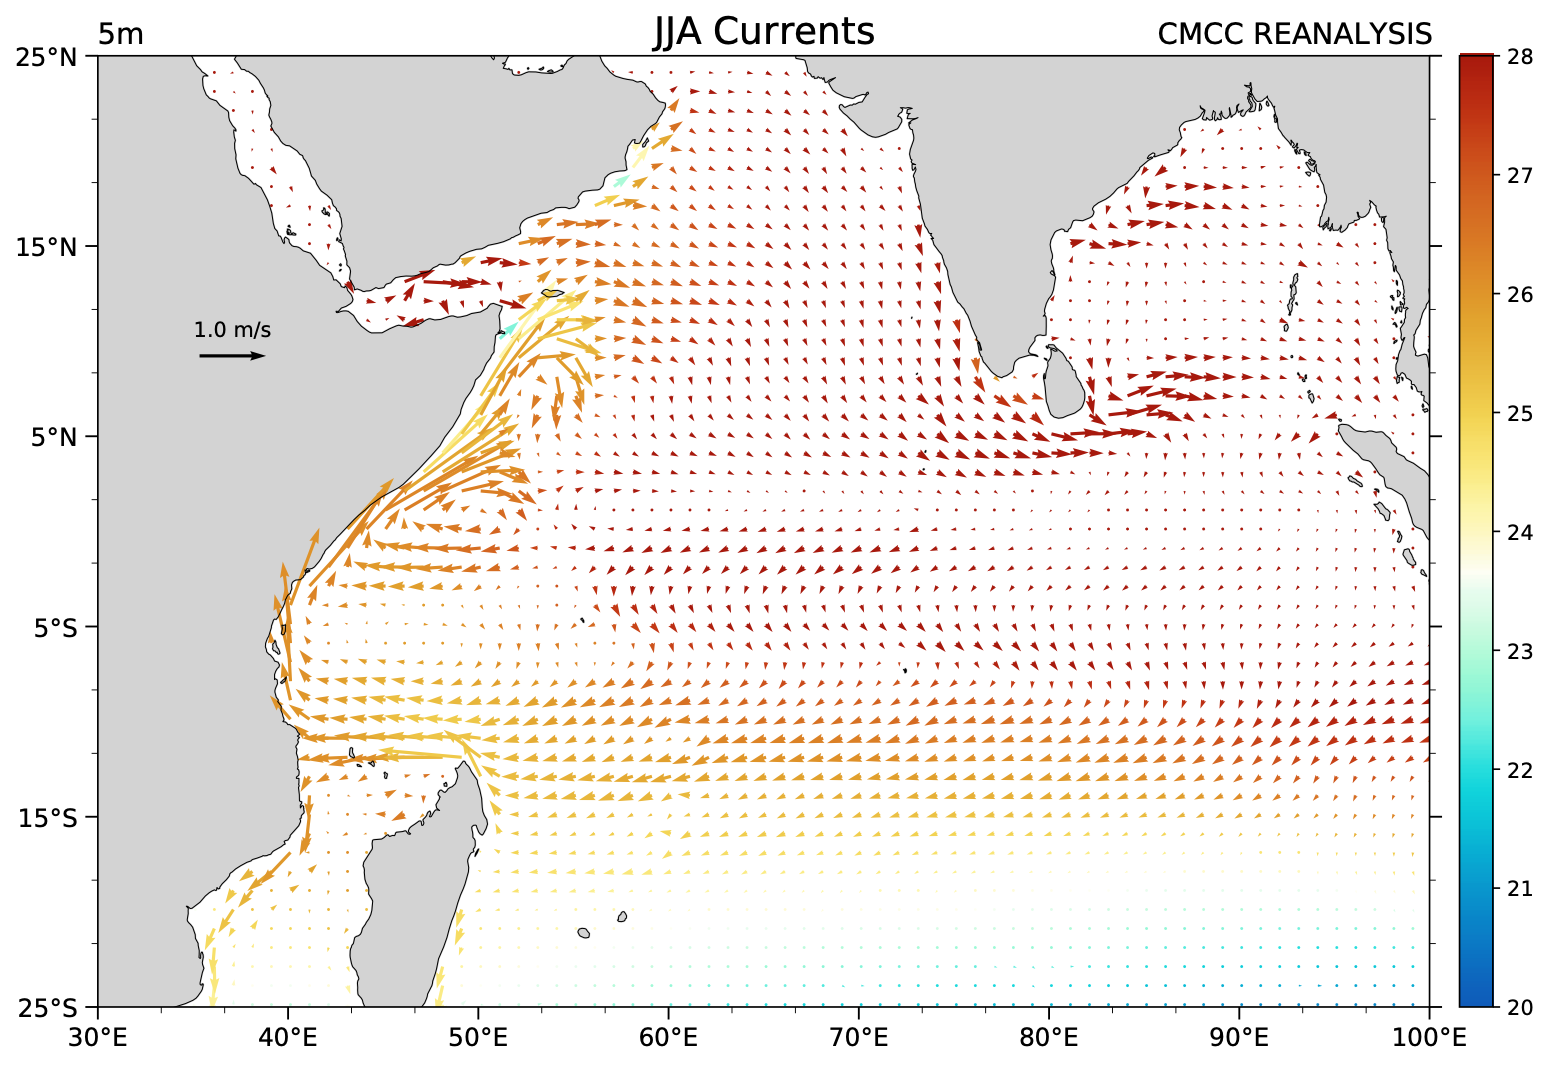
\includegraphics[width = 0.35\textwidth]{upload/46.png}
	\caption{The upwelling zones on the left and the Somali current on the right.} \label{fig:upwelzone}
\end{figure}




\section{Ice}
Sea ice covers about $7$\% of Earth's oceans and plays a critical role in the global climate system, acting as a barrier between the atmosphere and the ocean. It forms when seawater cools below its freezing point, creating ice floes that are often cracked and shifted by environmental forces. Despite its compact appearance, sea ice is dynamic and never fully covers open water areas due to constant movement and deformation. \\
In the Southern Hemisphere, sea ice extends seasonally from about $3$ million km\(^2\) in summer to $18$ million km² in winter, covering around $7$\% of the Southern Ocean at its peak. The ice can reach as far as $60°$S during winter, particularly in the Weddell and Ross Seas. However, it tends to be less compact compared to the Arctic, largely due to divergent winds and the influence of ocean currents. By contrast, in the Northern Hemisphere, sea ice ranges from $7$ million km\(^2\) in summer to $15$ million km² in winter, making up about $10$\% of the ocean area during its maximum extent. The Arctic Ocean forms the core region of sea ice, with thick polar caps and thinner ice in surrounding seas like the Bering Sea and the Sea of Okhotsk. Ice can also drift into the North Atlantic through the Labrador and Greenland seas.
The formation of sea ice depends on several factors. Salinity plays a crucial role, as higher salinity lowers the freezing point of seawater. In regions with salinity levels above $24.7$\%, convective mixing occurs as dense, salty water sinks, delaying the freezing process. Under calm conditions, supercooling can allow water to remain liquid below its freezing point until ice crystals form, which then accelerate the freezing of surrounding water. As the ice thickens, it insulates the ocean below, reducing heat loss and slowing further growth. \\
Sea ice melts during summer, particularly in the Arctic, where increased sunlight and prolonged daylight accelerate the process. Melting can occur at rates of about $40$ mm per day, with melt ponds and drainage channels forming on the surface. The loss of ice is further aided by tidal forces and storms, leading to disintegration near coastlines and open water areas. By late summer, much of the peripheral sea ice in the Arctic disappears, leaving only the central ice pack. \\
Sea ice properties vary greatly between the Arctic and Antarctic regions. In the Arctic, central ice thickness typically ranges from $2$ to $4$ meters, with thinner ice in peripheral seas ($0.5$ to $1$ meter). Antarctic icebergs are far larger, often exceeding $600$ meters in thickness. Ice density, generally between $880$ and $910$ kg/m\(^3\), allows it to float. The topography of sea ice includes ridges and rubble zones formed by colliding ice sheets, with some ridges extending $10$ to $15$ meters below the surface. \\
The movement of sea ice is also an important factor in ocean circulation and climate. In the Arctic, the Beaufort Gyre and the Transpolar Drift Stream transport ice across the Arctic Basin, eventually exiting through the Fram Strait into the North Atlantic. This ice contributes to cold currents like the East Greenland Current. In the Antarctic, ice drifts clockwise in the Weddell Sea, eventually melting in warmer waters and transporting freshwater to lower latitudes. \\
[0.15 cm]

Overall, sea ice is a vital component of Earth's climate system. It influences heat exchange between the ocean and atmosphere, regulates salinity and density in ocean waters, and contributes to the broader dynamics of polar and global ocean circulation. Its seasonal cycles and properties make it an essential focus for understanding climate change and its impacts.

\section{Interconnections between atmosphere, ocean and ice}
Important transfers of energy, mass, momentum occur between the oceans and the atmosphere and are greatly modified by the presence of sea ice.
\subsection{Atmosphere effect}
Wind forcing is a prime driver for upper ocean circulation and thereby impacts deep ocean circulation as well, and for sea ice thereby impacting its motions and location. In addition, air temperatures and moisture contribute to determining the energy fluxes across the interface between the atmosphere and surface, contributing to ice maintenance, growth and melt and to the temperature distribution in the ocean and water velocity.
Fridtjorf Nanse noted that sea ice does not drift in the direction of the wind but at an angle of $20-40°$ to the right due to the Earth’s rotation and speculated that the motions in the water beneath sea ice deviate even more; the motion of each water layer deviate slower and farther to the right to the layer above and Ekman proved it mathematically adding that these influence stops at a depth of about $200$ m.

\subsection{Ocean effect}
Ocean has a significant impact on the other two components. It is essentially a limitless moisture source and supplies the majority of atmospheric water vapor. The ocean land contrast exerts a major control over the distribution of evaporation over the global precipitation. The thermal inertia of the ocean results in a much lesser seasonal temperature range at the open ocean surface than at a land surface or a sea ice surface.
This creates a lesser atmospheric temperature range over open ocean than over land or sea ice, as cold winter air is warmed by the underlying ocean and warm summer air is cooled. %non ho capito fedeeeee
Since the ocean also absorbs a significant amount of the atmosphere’s carbon dioxide ($CO_2$), it also helps to slow the buildup of atmospheric $CO_2$. \\
[0.1 cm]
The oceans contribute significantly to the poleward transport of heat, by means of ocean currents. This transport influences the heat balances in both high and low latitudes and the average temperature gradient between the equator and the poles. The temperature distribution of the ocean surface is the prime determinant of the sea ice distribution, because, in general, ice forms where the water temperature has reached the freezing point. Similarly, the ocean salinity distribution is important to the formation of sea ice, because the salt content of the water affects the freezing temperature. Once ice is formed, warm currents entering an ice-covered region tend to melt the ice cover, and cold currents moving away from the ice region tend to carry ice with them.

\subsubsection{El Niño/Southern Oscillation (ENSO)}
This is an example of atmosphere/ocean interconnections one of the major large-scale patterns. The El Niño and Southern Oscillation phenomena were originally examined separately, before their close interconnection became apparent.\\
[0.1cm]
\textbf{El Niño} originally referred to a seasonal warming of the waters along the coast of Peru, frequently occurring shortly after Christmas. The term is now generally restricted to large-scale warming events, extending well into the central equatorial Pacific. The episodes can last many months, and do not necessarily begin near Christmas. \textbf{The Southern Oscillation}, characterized by consistent sea level pressure, temperature, and precipitation changes in the South Pacific, was first discussed by Walker who found an alternating pressure pattern involving the normal southeast Pacific high pressure and the low pressure region near the Indian Ocean and western Pacific regions. \\
[0,1cm]
\textit{Under normal conditions} (non–El Niño), there is a strong sea surface temperature difference between the warm western Pacific and the cooler eastern Pacific, caused by upwelling along South America's west coast driven by east-to-west trade winds. This setup creates a convection cycle where air rises over the warm western Pacific, leading to heavy rainfall, and sinks over the cooler eastern Pacific, forming an east-west Walker circulation.\\
\textit{During El Niño}, the trade winds weaken, reducing upwelling along the South American coast. This leads to warmer sea surface temperatures in the eastern Pacific, disrupting the temperature gradient. As a result, air rising and rainfall patterns shift eastward, cooling the western Pacific and causing significant climate effects. For example, the Indonesian-Australian region may experience drought, while wetter conditions occur farther east.
\begin{figure}[htpb]
	\centering
	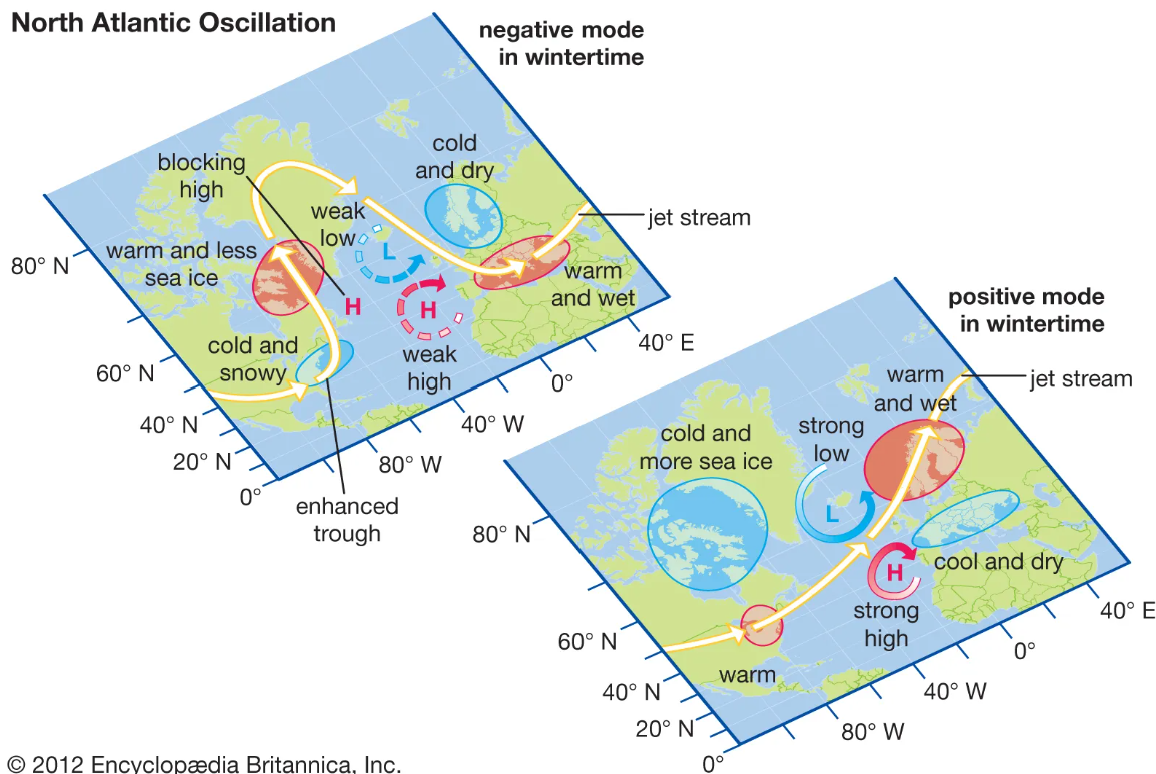
\includegraphics[width=0.5\linewidth]{upload/NAO.png}
	\caption{NAO}
	\label{fig:enter-label}
\end{figure}
\subsubsection{North Atlantic Oscillation (NAO)}
The North Atlantic Oscillation (NAO) is a pressure oscillation measured by the sea level pressure difference between Iceland and the Azores, reflecting the strength of the Icelandic low-pressure system and the Azores high-pressure system. (although sometimes it is indexed instead by the pressure difference between Newfoundland and Lisbon, Portugal, or between Iceland and Lisbon). It has both short-term and long-term variations, significantly affecting North Atlantic climate patterns. Positive NAO phases strengthen the Icelandic low pressure, resulting in colder winters in eastern North America, warmer and wetter conditions in western Europe, reduced sea ice near Greenland and Scandinavia, and increased sea ice in Baffin Bay and the Labrador Sea. \\
NAO impacts extend to global teleconnections, including influences on Russia, the Indian monsoon, and ocean temperatures. The positive NAO phase is associated with a tripolar sea surface temperature pattern: a cold anomaly in the subpolar North Atlantic, warm anomalies near Europe, and a cold subtropical anomaly near the Equator. The Gulf Stream further propagates these anomalies toward Europe, enabling atmospheric feedback and improving predictability of NAO patterns. The interaction between the ocean and the NAO remains a key area of research.



\subsection{Ice}
The presence of sea ice has numerous climatic consequences, influencing the temperature and circulation patterns of both the atmosphere and the oceans. Sea ice lessens the amount of solar radiation absorbed at the ocean's surface: only about $20–50$\% of the incident solar radiation is absorbed, the rest being reflected to space and is therefore lost, while without the ice, typically $85–95$\% is absorbed.
It serves as a strong insulator, restricting exchanges of heat from $10^2$ to $10^3 \,\,\text{Wm}^{-2}$  from the ocean to the atmosphere, to $10$ to $20 \,\,\text{Wm}^{-2}$;   mass, momentum, and chemical constituents between the ocean and atmosphere. \\
In winter, ice cover enhances polar cooling by increasing temperature gradients between the poles and the equator, intensifying atmospheric circulation. However, stronger circulation brings warm air into polar regions, reducing these gradients and creating a negative feedback, making the overall effect on atmospheric circulation uncertain. In summer, ice acts as a thermal insulator, reducing heat transfer from the atmosphere to the ocean. Its high albedo also reflects solar radiation, limiting heat absorption and increasing the net heat gain in polar oceans. These seasonal dynamics highlight the complex role of ice in the climate system.\\

Another aspect of the insulation is the lessened evaporative transfer to the atmosphere in the presence of ice cover, resulting in reduction of moisture available for cloud formation, rain and snow. \\
[0.1 cm]
The freezing and melting of sea ice influence seasonal and regional climates by moderating temperature extremes. Ice formation releases heat, while melting absorbs heat, facilitating a net equatorward transport of heat and salt from polar regions. During ice formation, salt is rejected into the underlying ocean, increasing the salinity and density of the mixed ocean layer, which can lead to deep convection and the formation of bottom water that drives global ocean circulation.
This process is most significant at the edges of ice packs, where winds create open water that freezes rapidly, enhancing local ice production. Approximately one-third of bottom water originates from ice formation along ice margins. These dynamics connect ice processes to global climate systems, influencing both local and large-scale ocean circulation.
